% !TeX root = main.tex
\documentclass[a4paper,fleqn]{cas-sc}
\usepackage[authoryear,longnamesfirst]{natbib}
\usepackage{csvsimple}
\usepackage{tikz}
\usepackage{tabularx}
\usepackage{pgfplots}
\usepackage{adjustbox}
\usepackage{placeins}
%%% Author definitions
\def\tsc#1{\csdef{#1}{\textsc{\lowercase{#1}}\xspace}}
\tsc{WGM}
\tsc{QE}
\tsc{EP}
\tsc{PMS}
\tsc{BEC}
\tsc{DE}

\begin{document}
\let\WriteBookmarks\relax
\def\floatpagepagefraction{1}
\def\textpagefraction{.001}

\shorttitle{Web Security Posture of Canadian Public-Sector Websites}
\shortauthors{I. Latta and S. Keshvadi}

\title [mode = title]{Policy Without Enforcement? Web Security Posture of Canadian Public-Sector Websites}

\tnotemark[1]
\tnotetext[1]{This work was supported by the CSA Group Undergraduate Research Scholarship.}

% First author
\author[1]{Isaac Latta}
\ead{latta11@mytru.ca}

\credit{Conceptualization, Methodology, Software, Data Curation, Investigation, Formal analysis, Visualization, Writing -- original draft}

\affiliation[1]{organization={Thompson Rivers University},
    addressline={805 TRU Way}, 
    city={Kamloops},
    state={British Columbia},
    postcode={V2C 0C8}, 
    country={Canada}}

% Second author (Corresponding)
\author[1]{Sina Keshvadi}
\cormark[1]
\ead{skeshvad@tru.ca}

\credit{Conceptualization, Methodology, Supervision, Writing -- review \& editing, Project administration}

\cortext[cor1]{Corresponding author}

% Footnotes for acknowledgments
\nonumnote{We gratefully acknowledge the support of the CSA Group Undergraduate Research Scholarship and thank CSA Group staff for their guidance during the project.}

% Abstract (Max 250 words)
\begin{abstract}
Public-sector websites are trusted entry points for high-consequence services, yet their security posture depends on layered controls that extend beyond HTTPS adoption. We present a standards-aligned, non-invasive measurement study of web security configuration across Canadian public-sector authority websites, compared against domestic critical sectors (finance, education, and energy) and peer public-sector datasets in the United States and United Kingdom. In this paper, we distinguish origin-scoped transport controls (HTTPS enforcement, TLS posture, HSTS, disclosure signaling) from endpoint-scoped browser protections (security headers and cookie attributes) to reflect how users experience security after redirects. Across 375 Canadian authority origins, foundational transport protections are widespread but uneven: only 59.73\% of HTTPS-reachable authority origins deploy HSTS, and authorities negotiate TLS 1.3 less frequently than comparable peers. Defense-in-depth is weakest at the application layer: modern policy headers (CSP frame-ancestors, Permissions-Policy) and hardened cookie defaults are rarely deployed. Only 1.1\% of Canadian authority origins publish security.txt, while reconnaissance surfaces remain common. These results indicate that the primary gap is inconsistent implementation of low-cost, configuration-driven controls. Cross-sector and cross-jurisdiction comparisons suggest that more enforceable governance environments are associated with more uniform adoption of defense-in-depth protections.
\end{abstract}

% Research highlights (3 to 5 bullets, max 85 chars per bullet)
\begin{highlights}
% \item Multi-layer evaluation methodology for automated public-sector web security scanning.
% \item Empirical analysis of 375 Canadian authority origins and critical-sector websites.
% \item Quantified performance gaps between recommendation- and mandate-driven models.
\item Foundational transport protections are widespread but uneven across Canadian public authorities: only 59.73\% deploy HSTS and TLS~1.3 is negotiated less frequently than in domestic critical sectors and international peers.
\item Defense-in-depth remains weakest at the application layer, with modern browser policy headers (CSP \texttt{frame-ancestors}, \texttt{Permissions-Policy}) and hardened cookie attributes rarely deployed, and only 1.1\% of authorities publishing \texttt{security.txt}.
\item Canadian authorities underperform both domestic critical sectors (finance, education, energy) and mandate-driven peers in the US and UK, indicating that recommendation-driven governance is associated with less consistent implementation of low-cost web security controls.

\end{highlights}

% Keywords (5 to 10 keywords)
\begin{keywords}
Web Security Measurement \sep Public-Sector Websites \sep Web Security Benchmarking \sep Security Headers \sep Internet measurement
\end{keywords}

\maketitle

\section{Introduction}~\label{sec:introduction}
    Public-sector websites have become a primary delivery channel for government information and services, enabling citizens to access essential resources, submit sensitive data, and make high-consequence decisions with legal, financial, and personal implications.
    In this context, security configuration directly shapes public trust, safety, and service continuity.
    The security posture of a modern web service is determined by multiple, interacting layers of controls, including transport protection (HTTPS/TLS), browser-enforced policies (e.g., HTTP Strict Transport Security (HSTS) and security response headers), secure session-management mechanisms (cookies), operational readiness for coordinated vulnerability disclosure, and disciplined suppression of implementation details that reduce attackers' reconnaissance advantage.
    % 
    HSTS, for example, is standardized in RFC~6797 and prevents SSL-stripping by enforcing HTTPS-only access at the user-agent level~\cite{rfc6797,mdn_sts_header}. Similarly, contemporary guidance recommends prioritizing TLS~1.3 and disabling legacy protocol versions due to known weaknesses and downgrade risks \cite{rfc8446,rfc8996,nist_800_52r2,nsa_eliminating_obsolete_tls,cccs-itsp-40062}. Beyond transport, defense-in-depth is achieved through browser-side hardening controls such as Content Security Policy (CSP), clickjacking protections, and Permissions-Policy \cite{owasp_http_security_response_headers,owasp_csp_cheatsheet,mdn_csp_guide}, alongside secure cookie attributes that mitigate token theft \cite{mdn_secure_cookie_configuration,owasp_session_management_cookies}. Finally, coordinated vulnerability disclosure is increasingly operationalized through standardized channels such as \texttt{security.txt} (RFC~9116), providing a low-cost mechanism to publish disclosure contacts \cite{rfc9116,cisa_securitytxt_simple_file_big_value}. Taken together, these layers imply that the practical question is no longer whether a site uses HTTPS, but whether it delivers robust, defense-in-depth protections across the web stack. 

    Across jurisdictions, approaches to securing public-sector web services vary in the extent to which best practices are enforced. The United States and the United Kingdom have increasingly adopted mandate-driven approaches, relying on enforceable instruments such as the U.S.\ HTTPS-only policy (OMB Memorandum M-15-13) and Binding Operational Directives (BODs), as well as the UK Government Digital Service (GDS) security standards \cite{omb-m-15-13,cisa_bod_18_01,gds_security_overview_websites}. In contrast, Canada operates primarily under a recommendation-driven model in which the Canadian Centre for Cyber Security (CCCS) issues technical guidance---for example, on securely configuring network protocols and related web-service protections---without an accompanying, centralized legal mandate that compels uniform adoption \cite{cccs-itsp-40062,cccs-itsm-60005}. This divergence motivates the central research question of this study: to what extent do Canadian authority websites implement these recommended best practices, and how does their implementation quality compare to other critical domestic sectors and international peers?

    This paper addresses this question through a large-scale, automated benchmarking study. We collected data from 375 Canadian authority origins and performed parallel data collection across Canadian critical sectors (finance, education, and energy) as well as the equivalent sectors in the United States and the United Kingdom. Our evaluation framework integrates CCCS guidance with widely adopted standards to assess: (i) transport-layer protections; (ii) application-layer hardening; (iii) information-disclosure surfaces, including technology-revealing headers and error handling \cite{owasp_secure_headers_project,cwe_209}; and (iv) operational transparency via \texttt{security.txt} \cite{rfc9116}. A key design choice in our measurement is to distinguish \emph{origin-scoped} controls (e.g., TLS configuration and HTTPS enforcement) from \emph{endpoint-scoped} controls (e.g., security headers and cookie attributes observed at the final resolved landing page), to reflect on how protections are applied at different layers of the web stack.

    Our findings indicate that although Canadian public-sector sites have broadly adopted foundational transport controls, they lag behind both international peers and domestic critical sectors in deploying more advanced defense-in-depth protections. This paper makes the following contributions:

    \begin{enumerate}
    % \item We develop and validate a multi-layer evaluation methodology that operationalizes security specifications from the Canadian Centre for Cyber Security (CCCS) alongside OWASP and MDN guidance into an automated scanning framework.
    % \item We present the first large-scale empirical analysis of the Canadian public-sector web ecosystem, evaluating 375 authority origins alongside critical sectors such as finance, education, and energy.
    % \item We conduct an empirical measurement study that quantifies differences between Canada's recommendation-driven governance model and the mandate-driven models employed in the United States and the United Kingdom.
    \item Foundational transport protections are widespread but uneven across Canadian public authorities: only 59.73\% deploy HSTS and TLS~1.3 is negotiated less frequently than in domestic critical sectors and international peers.
\item Defense-in-depth remains weakest at the application layer, with modern browser policy headers (CSP \texttt{frame-ancestors}, \texttt{Permissions-Policy}) and hardened cookie attributes rarely deployed, and only 1.1\% of authorities publishing \texttt{security.txt}.
\item Canadian authorities underperform both domestic critical sectors (finance, education, energy) and mandate-driven peers in the US and UK, indicating that recommendation-driven governance is associated with less consistent implementation of low-cost web security controls.
\end{enumerate}


The remainder of the paper is organized as follows. Section~\ref{sec:background} reviews background and related work. Section~\ref{sec:methodology} describes dataset construction, measurement units and preprocessing, the standards-aligned security tests, and scanner implementation and validation. Section~\ref{sec:results} presents results across transport security, browser-enforced controls, disclosure readiness, and information leakage. Section~\ref{sec:discussion} discusses implications for operators and policymakers and summarizes study limitations. Section~\ref{sec:conclusion_future} concludes the paper and outlines directions for future work.


\section{Background and Related Work}~\label{sec:background}
    \subsection{Background}
    The security posture of a modern web service is a composite of multi-layered controls designed to provide defense-in-depth. In this paper, we categorize these controls into three functional domains: transport-layer security, application-layer hardening, and operational transparency.

    \paragraph{Transport-Layer Security}
    HTTPS protects the confidentiality and integrity of data in transit by layering HTTP over the Transport Layer Security (TLS) protocol. However, the presence of HTTPS alone does not guarantee a secure state. Misconfigurations, such as supporting weak cipher suites or legacy protocols (e.g., TLS 1.0 and 1.1), expose users to downgrade attacks and cryptographic interception~\cite{rfc8996}. Contemporary best practices, as defined by NIST and the CCCS, prioritize TLS 1.3 to leverage modern cryptographic primitives~\cite{rfc8446, nist_800_52r2, cccs-itsp-40062}. Furthermore, HTTP Strict Transport Security (HSTS) is a critical policy mechanism (RFC 6797) that instructs browsers to interact with a domain exclusively over HTTPS, mitigating SSL-stripping and preventing users from bypassing certificate warnings~\cite{rfc6797, mdn_sts_header}.

    \paragraph{Application-Layer Hardening} 
    Modern browsers enforce a sophisticated suite of security policies delivered via HTTP response headers to mitigate application-level vulnerabilities. Central to this defense-in-depth approach is the Content Security Policy (CSP), a robust framework for constraining resource loading, such as scripts and frames, which serves as a primary mitigation against Cross-Site Scripting (XSS) and various data injection vectors~\cite{owasp_csp_cheatsheet, mdn_csp_guide}. These browser-side protections are further augmented by headers designed to prevent interface manipulation and content misinterpretation. For instance, \texttt{X-Frame-Options} and \texttt{X-Content-Type-Options: nosniff} are utilized to defend against clickjacking and MIME-sniffing attacks, respectively~\cite{owasp_http_security_response_headers}. Furthermore, since cookies remains the dominant mechanism for state management, the resilience of a web service to session hijacking is largely determined by their configuration. Attributes such as \texttt{Secure}, which restricts transmission to encrypted channels, \texttt{HttpOnly}, which prevents script-based token access, and \texttt{SameSite}, which limits cross-site request behavior, are essential for neutralizing session compromise pathways like token theft and Cross-Site Request Forgery (CSRF)~\cite{mdn_secure_cookie_configuration, owasp_session_management_cookies}.

    \paragraph{Operational Transparency and Information Governance} 
    Beyond active technical defenses, the reduction of an organization's attack surface necessitates disciplined information governance and operational transparency. Unintentional disclosure of implementation details, such as technology-revealing \texttt{Server} or \texttt{X-Powered-By} headers and verbose error pages, provides attackers with a significant ``reconnaissance advantage'' by facilitating low-effort fingerprinting of the underlying software stack~\cite{owasp_secure_headers_project, cwe_209}. Conversely, a high degree of operational maturity is signaled by the proactive adoption of standardized vulnerability disclosure channels. RFC~9116 defines \texttt{security.txt}, a machine-readable file placed at a well-known path that allows security researchers to report vulnerabilities efficiently and securely. This mechanism is increasingly advocated by international authorities, including CISA and the CCCS, as a low-cost yet high-impact step to strengthen national incident-response ecosystems and reduce the time-to-triage for discovered security flaws~\cite{rfc9116, cisa_securitytxt_simple_file_big_value, cccs-itsm-60005}.

    % Government and industry profiles further operationalize these expectations through configuration guidance, including NIST recommendations for TLS selection and deployment~\cite{nist_800_52r2} and national guidance on detecting and eliminating obsolete TLS configurations~\cite{nsa_eliminating_obsolete_tls}.
    % In Canada, CCCS guidance similarly provides concrete protocol configuration recommendations, including TLS version prioritization and acceptable cryptographic profiles~\cite{cccs-itsp-40062}.

    \subsection{Related Work}
    Prior research into public-sector web security has primarily focused on large-scale HTTPS adoption and transport-layer configurations, yet these studies vary significantly in jurisdictional focus, measurement granularity, and the breadth of controls evaluated.
    
    % Government and public-sector web posture measurement
    Empirical assessments of government web services have traditionally targeted single-nation populations or specific regulatory frameworks. 
    Dunbar et al.\ proposed a scoring methodology for U.S.\ domains based on SSL/TLS support and HSTS presence, noting that advanced features like HSTS were infrequently deployed despite federal guidance~\cite{dunbar4240917survey}. 
    Similarly, Schiavone et al.\ analyzed the adoption of transport security across 8,000 Italian municipality websites, finding that compliance with national regulations varied systematically by region and demographic profile~\cite{schiavone2024municipality2https}. 
    Beyond simple configuration, Hsiao et al.\ explored the concept of ``cyber autonomy'' among G7 government websites, revealing a high degree of dependence on third-party infrastructure and demonstrating how different policy environments—particularly centralized mandates—directly influence security adoption outcomes~\cite{hsiao2019cyberautonomy}.
    
    % Automated scanners and practitioner tooling
    A distinct body of literature focuses on the development of scanners for assessing specific web security layers. 
    At the transport layer, platforms such as SSL Labs and longitudinal trackers like SSL Pulse provide Internet-scale insights into protocol support and cipher hygiene~\cite{tool_ssllabs_ssltest,SSLPulse}. 
    For application-layer hardening, tools such as Mozilla's HTTP Observatory and SecurityHeaders.com provide header-focused grading for individual endpoints~\cite{tool_mozilla_observatory,tool_securityheaders}. 
    While these platforms are invaluable for site-specific diagnostics, they are generally not designed for the systematic, multi-sector benchmarking of curated populations. 
    Furthermore, existing scanners often treat security posture as a monolithic domain attribute, frequently failing to distinguish between transport properties at the host origin and application controls observed at final landing pages after a redirect chain.
    
    % Gaps addressed by this study
    Despite these advancements, the Canadian public-sector ecosystem remains significantly understudied. 
    Most longitudinal analyses emphasize the U.S.\ and European landscapes, where binding mandates (e.g., BOD 18-01) often dictate security requirements. 
    This leaves a critical gap in understanding how a recommendation-driven model, such as Canada's, performs in comparison to mandate-driven peers. 
    Moreover, few studies integrate transport security, browser-side policy controls (CSP/HSTS), and operational disclosure readiness into a single unified framework aligned to specific national guidance. 
    This paper addresses these gaps by providing a comparative analysis of Canadian authority and critical-sector websites against their U.S.\ and U.K.\ counterparts, utilizing a non-invasive scanner designed to operationalize CCCS, OWASP, and MDN specifications~\cite{cccs-itsp-40062,cccs-itsm-60005,owasp_http_security_response_headers,mdn_sts_header}.

    % Methodology section
\section{Methodology}~\label{sec:methodology}
% one opening paragraph about Study Design Overview
    This section describes the methodology used to construct our measurement datasets and to evaluate the web security posture of public-sector and critical-sector websites. 
    We first define the target populations and explain how we compiled representative website lists for each sector and jurisdiction from authoritative sources. 
    We then formalize the measurement units used throughout the study (URI, origin, and endpoint) and describe the preprocessing steps required to canonicalize targets and resolve redirects to the final measurable destinations. 
    Next, we present the set of security controls evaluated by our scanner, explicitly distinguishing origin-scoped controls (e.g., transport and TLS configuration) from endpoint-scoped controls (e.g., browser-enforced headers and cookie attributes), as well as auxiliary probes for vulnerability disclosure and information leakage. 
    Finally, we summarize the scanner implementation, ethical rate-limiting constraints, and validation procedures used to ensure the accuracy and reliability of automated classifications, along with the approach used to aggregate and analyze results across datasets.

\subsection{Target Populations and Dataset Construction}
    We study four sectors whose public-facing web services either deliver core government functions or support critical societal infrastructure: (i) \emph{public authorities} (government departments, agencies, and public bodies), (ii) \emph{finance} (banks and credit unions), (iii) \emph{education} (universities and colleges), and (iv) \emph{energy} (electricity, oil/gas pipelines, and nuclear-related facilities).
    To contextualize Canadian deployment patterns, we construct comparable datasets from the United States and the United Kingdom where authoritative sources are available.
    Targets were assembled from authoritative registries, APIs, and official sector lists.
    Candidate URLs are later canonicalized and deduplicated through the preprocessing pipeline described in Section~\ref{sec:measurement_units}, to ensure that multiple source entries referring to the same hosted service are counted consistently.
    We include only \emph{public-facing} web services intended for citizen, customer, or stakeholder access.
    
    For Canada, authority websites are compiled from federal and provincial public directories and official listings, supplemented where necessary by regulator-maintained registries~\cite{canada_depts,canada_institutions,crown_corps,ca_airports,maritime_ports,ca_emergency_management}.
    For Canadian finance, we include Schedule I and II member banks listed by the Canadian Bankers Association (CBA), complemented by provincial credit-union registries where authoritative listings are available~\cite{cba_member_banks_2024}.
    For Canadian education, we use the Universities Canada membership list to identify public-facing universities and colleges~\cite{ca_unis_list}.
    For Canadian energy, we use Electricity Canada’s member list for the electricity sector, and regulator-maintained registries for interprovincial/international pipeline operators and licensed nuclear facilities~\cite{electric_canada_members,cer_pipeline_companies,cnsc_nuclear_facilities}.
    Where relevant, we also use sector association listings to capture additional operators (e.g., natural gas distribution entities)~\cite{cga_industry_links}.
    
    For U.S.\ public authorities, we use the USA.gov agency index, which provides canonical contact and website references for federal entities~\cite{usa-agency-index}.
    For U.S.\ finance, we use the FDIC BankFind Suite API, which provides institution records including primary internet web addresses~\cite{fdic-bankfind-api}.
    For U.S.\ education, we use the U.S.\ Department of Education College Scorecard API, which provides institution-level records suitable for systematic sampling~\cite{us-college-scorecard-docs}.
    
    For UK public authorities, we use the GOV.UK organisations endpoint (and related collections infrastructure) to obtain organisation records and associated public web presences~\cite{uk-gov-collections-api,uk-gov-collections-api-docs}.
    For UK finance, we use the Bank of England’s PRA-regulated banks list as the primary registry of regulated banks~\cite{uk-pra-creditunions-list}.
    For UK education, we use the Discover Uni (formerly Unistats) dataset, which provides official provider/course metadata distributed by HESA and partner bodies~\cite{hesa_discoveruni_2024}.
    For the UK, we include public authorities, finance, and education, and we omit UK energy because we did not identify a single authoritative registry that consistently publishes complete, URL-resolvable website fields for that sector.

    Some source registries contain very large populations (notably U.S.\ finance and education).
    In those cases, we use a sampling strategy to retain geographic and institutional diversity while keeping measurement feasible at scale.
    Table~\ref{tab:dataset_sources} summarizes the resulting datasets (sizes by sector and jurisdiction) and the primary sources used to construct each list.


\begin{table}[t]
  \caption{Overview of website datasets and primary data sources.}
  \label{tab:dataset_sources}
  \centering
  \scriptsize
  \setlength{\tabcolsep}{3pt}
  \renewcommand{\arraystretch}{1.15}
  \begin{tabularx}{\columnwidth}{l l X}
  \toprule
  Country & Sector & Primary data sources \\
  \midrule
  Canada & Authorities &
  Compiled from Government of Canada official directories of departments and federal institutions
  \cite{canada_depts,canada_institutions}; remaining provincial authority lists were obtained from
  official provincial directories (manual lookup where no consolidated registry exists). \\
  Canada & Finance &
  Schedule I and II banks from the Canadian Bankers Association \cite{cba_member_banks_2024};
  credit unions from provincial regulator registries (manual consolidation). \\
  Canada & Education &
  Public-facing universities and colleges from Universities Canada \cite{ca_unis_list}. \\
  Canada & Energy &
  Electricity sector from Electricity Canada member list \cite{electric_canada_members};
  oil/gas and nuclear from federal regulator registries \cite{cer_pipeline_companies,cnsc_nuclear_facilities}. \\
  \addlinespace[0.4em]
  USA & Authorities &
  Federal agency index of U.S. government organizations \cite{usa-agency-index}. \\
  USA & Finance &
  FDIC ``BankFind'' API \cite{fdic-bankfind-api}; sampling by ten most populous states based on
  U.S.\ population statistics \cite{us-population-stats}. \\
  USA & Education &
  U.S.\ Department of Education ``College Scorecard'' API \cite{us-college-scorecard-docs};
  sampling by ten most populous states based on U.S.\ population statistics \cite{us-population-stats}. \\
  USA & Energy &
  Edison Electric Institute list of member companies and their websites \cite{edison-electric-member-sites}. \\
  \addlinespace[0.4em]
  UK & Authorities &
  GOV.UK Collections API (organization listings, filtered to ``live'') \cite{uk-gov-collections-api-docs}. \\
  UK & Finance &
  Bank of England PRA-regulated banks list \cite{uk-pra-creditunions-list} cross-referenced against
  the FCA FSDeveloper API \cite{uk-fca-api-docs}. \\
  UK & Education &
  Discover Uni dataset of higher-education providers \cite{hesa_discoveruni_2024}. \\
  UK & Energy &
  No dataset was constructed; we did not identify an authoritative, URL-complete registry of UK energy providers. \\
  \bottomrule
  \end{tabularx}
\end{table}

\subsection{Measurement Units and Preprocessing}\label{sec:measurement_units}
% Measurement units: URI, origin, and endpoint    
Throughout this study, we distinguish between three related units of analysis: \emph{URIs}, \emph{origins}, and \emph{endpoints}.
    A \emph{URI} refers to the input web address obtained from a registry or directory and may include a scheme, host, optional port, and a path (and in some cases query parameters).
    An \emph{origin} is defined as the tuple \texttt{scheme + host + port} and represents the configuration boundary for transport-layer controls (e.g., TLS negotiation behavior and HSTS policy).
    An \emph{endpoint} refers to a user-reached URI after following redirects and includes the path component. Endpoint-level responses are where browser-facing policies (e.g., security headers and cookie attributes) are observed.
    This distinction is central to our measurement design as some controls are naturally origin-scoped (transport security and disclosure mechanisms), while others are endpoint-scoped (browser-enforced policies and session attributes). 

    % Canonicalization of candidate targets
    Input targets from source registries are first normalized to ensure consistent counting and to reduce duplicate measurement of the same hosted service.
    Hostnames are lowercased, and default ports are removed (80 for HTTP and 443 for HTTPS).
    Where an input omits an explicit scheme, we assign \texttt{https://} as the default to reflect modern expectations for public web services.
    For origin-scoped evaluation, we strip paths and queries to derive the canonical origin; for endpoint-scoped evaluation, we retain the full URI to reflect the page a user agent ultimately receives.

    % Redirect resolution and consolidation
    After canonicalization, we perform a redirect-resolution pass to map each input URI to the final user-reached destination.
    For each candidate URI, the scanner issues an HTTP \texttt{GET} request and examines the response status code.
    Any non-3xx response (e.g., \texttt{200 OK}, \texttt{403 Forbidden}) is treated as the final response.
    For 3xx responses with a \texttt{Location} header, the scanner follows the redirect target, recording each hop (status code and target URL) until a final non-3xx response is reached.
    To prevent unbounded redirect loops and to keep measurement non-invasive, we stop resolution if the chain exceeds a fixed hop limit (8 hops) or if a redirect response omits a \texttt{Location} header; such cases are tagged as resolution errors rather than followed indefinitely. 
    
    % De-duplication and measured target sets
    Redirect resolution yields two de-duplicated measurement sets.
    First, we derive a set of \emph{unique origins} for origin-scoped tests by extracting origins from both the entry and final resolved destinations and de-duplicating across the combined set.
    Second, we derive a set of \emph{final resolved endpoints} for endpoint-scoped tests, using only the final URI after redirects (since this reflects what end users and browsers actually interact with).
    This design ensures that transport-layer posture is measured at the correct configuration boundary, while browser-enforced controls are measured on the user-reached response.
% 
    % Implications of consolidation (e.g., centralized hosting)
    Redirect resolution can substantially consolidate apparent populations when multiple directory-listed URLs ultimately converge on a small number of shared final origins (e.g., centralized government hosting).
    We explicitly report both pre-resolution and post-resolution counts (input URIs, final URIs, input origins, and unique measured origins) to make this consolidation transparent and to avoid over-counting replicated services.

    % Non-goals and scope limitations (threat model boundaries)
    Our preprocessing and subsequent measurements are designed to characterize observable configuration posture and information exposure, not to discover or exploit vulnerabilities.
    Accordingly, we do not perform authenticated crawling, do not submit forms or issue state-changing requests (e.g., \texttt{POST}), and do not run exploit payloads or intrusive fuzzing.
    All findings should therefore be interpreted as indicators of standards-aligned control adoption and observable leakage at the network and HTTP layers, rather than as a full security audit of each service.

    \subsection{Security Control Tests}\label{sec:security_control_tests}

    For each target derived from the preprocessing pipeline (Section~\ref{sec:measurement_units}), the scanner applies a suite of tests that operationalize guidance from the Canadian Centre for Cyber Security (CCCS), relevant IETF RFCs, and widely adopted web-security recommendations (OWASP and MDN). 
    Tests are grouped by the security layer they target and by their natural measurement scope: origin-scoped controls are evaluated at the \texttt{scheme+host+port} boundary, while endpoint-scoped controls are evaluated on the final user-reached URI after redirects. 
    Across all modules, probes are designed to be non-invasive and rely only on standard protocol interactions and response parsing (no payload injection or authenticated crawling).

    \subsubsection{Transport Controls (origin-scoped)}\label{sec:transport_controls}
    % HTTPS reachability and HTTP$\rightarrow$HTTPS upgrade
    We first measure baseline transport protections: HTTPS reachability, HTTP-to-HTTPS upgrade behavior, and HSTS deployment. For each origin, the scanner attempts connectivity over both \texttt{http://} and \texttt{https://}. To evaluate HTTPS-only enforcement, we issue an HTTP request and determine whether the origin upgrades the user to HTTPS via a redirect chain whose terminal URI uses the \texttt{https} scheme.
    We additionally record cases where HTTP responds without upgrade, since these represent user-accessible cleartext entry points.

    To evaluate HTTP Strict Transport Security (HSTS), we check for the presence of the \texttt{Strict-Transport-Security} response header on HTTPS responses, as defined in RFC~6797~\cite{rfc6797}. When present, we parse the policy directives, including \texttt{max-age}, \texttt{includeSubDomains}, and \texttt{preload}. Following common operational practice and browser preload requirements, we classify an HSTS configuration as \emph{strong} when it specifies a long \texttt{max-age} (at least one year) and includes subdomain coverage (i.e., \texttt{includeSubDomains}). We separately record preload signalling. These transport controls are treated as origin-scoped because they govern connection security and user-agent upgrade behavior at the origin level.


\subsubsection{TLS Configuration (origin-scoped)}\label{sec:tls_configuration}
% Protocol version support
    Beyond HTTPS availability, we profile each origin's Transport Layer Security (TLS) posture to determine
    (i) which protocol versions the service supports and 
    (ii) which version is negotiated by a modern client in practice. 
    TLS~1.3 is standardized in RFC~8446, and legacy TLS~1.0 and TLS~1.1 have been formally deprecated due to limited support for modern cryptography and increased downgrade risk (RFC~8996)~\cite{rfc8446,rfc8996}. CCCS guidance similarly recommends prioritizing modern TLS configurations and disabling obsolete protocol versions \cite{cccs-itsp-40062}.
    
    % Negotiated version under a ``natural'' handshake
    For each origin, the scanner attempts constrained handshakes for TLS~1.3, TLS~1.2, TLS~1.1, and TLS~1.0 to record protocol support (success/failure per version). 
    To approximate what typical users receive, we also perform a single \emph{natural} handshake using a modern client configuration and record the negotiated protocol version. We report negotiated TLS versions rather than attempting to infer security from certificate properties or application-layer behavior, as our goal is to measure externally observable deployment posture at the transport layer.

% ------------------------------------------------------------
% Optional (kept for reviewer requests): TLS 1.2 cipher analysis
% ------------------------------------------------------------
% In addition to protocol versions, TLS configuration quality can be assessed by examining negotiated
% cipher suites (particularly for TLS~1.2). If enabled, the scanner can record the cipher suite
% selected during the natural handshake and/or perform a forced TLS~1.2 handshake to capture the
% negotiated cipher suite, then classify suites into guideline-derived categories (e.g., recommended,
% sufficient, phase-out) based on CCCS and allied guidance. This provides finer-grained visibility into
% cryptographic choices where TLS~1.2 remains in use, but requires careful mapping between observed
% cipher identifiers and the referenced policy categories.

\subsubsection{Browser-Enforced Policies (endpoint-scoped)}\label{sec:browser_policies}

    We next evaluate browser-enforced security policies implemented via HTTP response headers on the final resolved landing-page endpoint. 
    These controls provide defense in depth by constraining browser behavior even when application-layer weaknesses exist. 
    Guided by OWASP and MDN recommendations, we record the presence of the following headers on the final endpoint response~\cite{owasp_http_security_response_headers,mdn_csp_guide}:

    \begin{itemize}
    \item \texttt{Referrer-Policy}, which limits cross-origin referrer leakage and can reduce inadvertent disclosure of sensitive URL paths or parameters.
    \item \texttt{X-Content-Type-Options: nosniff}, which mitigates MIME-sniffing and content-type confusion behaviors in browsers.
    \item Clickjacking defenses via either \texttt{X-Frame-Options} or \texttt{Content-Security-Policy} framing restrictions. Because CSP offers the modern framing control, our CSP analysis focuses specifically on whether a \texttt{Content-Security-Policy} header includes the \texttt{frame-ancestors} directive; we record \texttt{X-Frame-Options} as a legacy but still-deployed control.
    \item \texttt{Permissions-Policy}, which restricts access to powerful browser features (e.g., camera, microphone, geolocation) and can reduce privacy and abuse surface in composite applications.
    \end{itemize}
    These tests are endpoint-scoped because header policies may vary by path, application component, or response type, and the final landing page represents the most consistent user-facing entry point for comparative measurement.

\subsubsection{Session Cookie Attributes (endpoint-scoped)}\label{sec:cookies}
    Because cookies frequently carry session identifiers and user state, we measure baseline cookie-hardening attributes on the final endpoint response. 
    For endpoints that set cookies (i.e., responses containing one or more \texttt{Set-Cookie} headers), we parse cookie attributes and record whether cookies include: 
    (i) \texttt{Secure} (restrict transmission to HTTPS), (ii) \texttt{HttpOnly} (restrict JavaScript access), and (iii) \texttt{SameSite} (restrict cross-site sending). 
    These attributes are widely recommended as baseline session protections~\cite{mdn_secure_cookie_configuration,owasp_session_management_cookies}.

    To summarize adoption, we compute attribute prevalence among cookie-setting endpoints and classify cookie posture using a simple rule set: endpoints are considered \emph{recommended} when cookies include \texttt{Secure} and \texttt{HttpOnly} and enforce a strict cross-site policy (e.g., \texttt{SameSite=Strict}); \emph{sufficient} when \texttt{Secure} and \texttt{HttpOnly} are present with \texttt{SameSite=Lax} or stronger; and otherwise \emph{insufficient}. 
    Because cookie behavior can vary across application paths and user states, this study evaluates cookies on the public landing response only, and interprets results as an indicator of baseline hygiene rather than a complete session audit.

\subsubsection{Vulnerability Disclosure (origin-scoped)}\label{sec:securitytxt}
    We assess operational readiness for coordinated vulnerability disclosure by probing for \texttt{security.txt}, a standardized, machine-parsable disclosure file defined in RFC~9116~\cite{rfc9116}. 
    For each origin, the scanner issues \texttt{GET} requests to both \texttt{/.well-known/security.txt} (preferred location) and \texttt{/security.txt} (legacy location). 
    A response is treated as a candidate \texttt{security.txt} file if it returns \texttt{200 OK} and contains minimally valid disclosure information (e.g., at least one \texttt{Contact:} field and/or a syntactically valid \texttt{Expires:} field). 
    When present, we record field completeness (e.g., presence of \texttt{Contact}, \texttt{Expires}, and optional \texttt{Canonical}) and treat expired \texttt{Expires} values as operationally weak because they indicate outdated disclosure metadata. 
    This test is origin-scoped because disclosure practices are typically managed at the site/operator level and are conventionally published per domain.

\subsubsection{Information Leakage (endpoint + error-path probe)}\label{sec:info_leakage}
    Finally, we measure two forms of low-effort fingerprinting surface that commonly arise from configuration defaults: (i) technology-revealing response headers and (ii) error-handling disclosures. 
    First, on the final endpoint response we check for the presence of headers that advertise server software, frameworks, or platforms (e.g., \texttt{Server}, \texttt{X-Powered-By}), using a curated list derived from OWASP guidance on removing revealing headers~\cite{owasp_secure_headers_project}. 
    When such headers are present, we additionally flag whether values appear to disclose explicit version strings, since version leakage can lower attacker reconnaissance cost and accelerate vulnerability targeting.

    Second, to evaluate error-handling disclosure in a safe and consistent way, the scanner requests a deliberately non-existent path on each origin (a randomized tokenized 404 probe) to trigger the site's default error handler without sending exploit payloads. If the response returns textual content, we analyze the body for technology and version indicators using signature-based matching (e.g., common framework banners and version formats) and report whether any technology identifiers are disclosed. We do not attempt to validate exploitability; these tests are intended to measure observable configuration and disclosure surfaces only.

\subsection{Scanner Implementation}
    The measurement pipeline was implemented as an automated scanner composed of modular probes corresponding to the control families described in Section~\ref{sec:security_control_tests}. 
    The scanner ingests the sector/jurisdiction target lists, applies the preprocessing pipeline (canonicalization and redirect resolution), and then executes the security-control modules in a fixed order while enforcing conservative resource limits to avoid disrupting production services.

    \paragraph{Architecture and execution model}
    The scanner is organized as a set of modular tests grouped by measurement scope. Preprocessing produces two deduplicated target sets: a unique \emph{origin} set for origin-scoped tests (e.g., HTTPS reachability, HSTS parsing, TLS probing) and a unique \emph{final endpoint} set for endpoint-scoped tests (e.g., security headers and cookie attributes). 
    Each module consumes only the target set relevant to its scope, writes structured results to disk, and emits summary counters for monitoring progress. 
    To improve throughput without overloading any individual service, the scanner uses bounded concurrency with both a \emph{global} concurrency limit and a \emph{per-origin} concurrency limit, to ensure that the scanner does not send bursts of requests to a single host.

    \paragraph{HTTP behavior and redirect handling}
    For all HTTP interactions, the scanner uses standard \texttt{GET} requests and processes responses according to the redirect resolution policy defined in Section~\ref{sec:measurement_units}. 
    Redirect chains are followed up to a fixed maximum depth; if a chain exceeds the maximum, the scanner records an error state and does not continue. For each input URI, the scanner records the full redirect chain (status codes and \texttt{Location} targets), the entry URI, and the final resolved URI. 
    The final resolved URI is then used as the canonical endpoint for endpoint-scoped tests, while origins derived from entry and final URIs form the origin set for origin-scoped tests.
    % cache
    To reduce unnecessary traffic and ensure consistent parsing, redirect-resolution outputs (final endpoint, redirect chain metadata, and response headers) are cached for reuse across modules, so that subsequent tests do not repeat identical resolution work.

    \paragraph{Rate limiting, timeouts, and stop rules (ethical scanning constraints)}
    All network interactions are bounded by client-side timeouts and conservative retry/stop rules. We impose a strict global limit on concurrent in-flight requests and a smaller per-origin limit, implemented using semaphores. In our deployment configuration, authority datasets were scanned with at most 15 concurrent requests globally and at most 3 concurrent requests per origin; the remaining sectors were scanned with at most 20 concurrent requests globally and at most 5 concurrent requests per origin. 
    Each HTTP request uses a 3-second timeout, and each TLS probing attempt uses a 3-second handshake timeout. 
    To avoid repeated probing of hosts that appear to block automated traffic or are persistently unreachable from the scanner's vantage point, the scanner maintains per-origin failure counters and stops further HTTP modules after 3 consecutive HTTP failures and stops further TLS modules after 2 consecutive TLS failures. 
    Origins that exceed these thresholds are marked as temporarily unavailable for the corresponding protocol and excluded from subsequent modules.

    \paragraph{TLS probing implementation}
    To measure protocol support, the scanner attempts constrained handshakes for TLS~1.3, TLS~1.2, TLS~1.1, and TLS~1.0 by configuring the client to offer only the targeted version and recording whether the handshake succeeds. To approximate the typical user experience, the scanner performs one additional \emph{natural} handshake using a modern client configuration and records the negotiated protocol version (and, if enabled, negotiated cipher suite). TLS probing does not attempt certificate-path validation beyond what is required to complete the handshake; the objective is to measure externally observable configuration posture rather than to act as a full PKI validation tool.

    \paragraph{Vantage point and scan window}
    Measurements were conducted from a single external scanning vantage point hosted on the Google Cloud Platform (GCP) within the us-central1 region.
    The results therefore represent a cross-sectional snapshot of observable posture. 
    The scanner records the scan start/end timestamps, software version, and configuration parameters (timeouts, concurrency limits, redirect depth, stop thresholds) to support reproducibility and interpretation of unreachable outcomes. 
    Where services rate-limit, geofence, or block automated clients, our conservative stop rules capture this as an externally observable availability constraint rather than attempting to bypass defenses.

    \paragraph{Output artifacts and reproducibility}
    Each module emits machine-readable results (per-origin and per-endpoint records) along with aggregate summaries used in the Results section. 
    Intermediate artifacts produced by preprocessing (canonicalized URIs, redirect chains, and deduplicated origin/endpoint sets) are retained to enable auditing of denominators and to support re-analysis. The scanner configuration (sector-specific concurrency limits, timeouts, and stop thresholds) is treated as part of the experimental setup and is documented alongside the results.
    % git
    The full source code of our automated scanner, along with the raw measurement datasets and sector-specific target lists, are publicly available on GitHub~\cite{latta_scanner_2026}.

%%%%%%%%%%%%%%%%%%%%%%% Extra text by Issac
% The first evaluation tests whether each origin actually supports HTTPS and whether it enforces HTTPS 
% in line with modern guidance. This is an origin-scoped test, as HTTPS/HTTP operate at the transport layer. 
% The CCCS outlines in
% ITSP.40.062 \cite{cccs-itsp-40062} and ITSM.60.005 \cite{cccs-itsm-60005}, that origins should not only support HTTPS, 
% but also implement HTTP Strict Transport 
% Security (HSTS) as outlined in RFC 6797 \cite{rfc6797}. HSTS informs the browser that this origin should \emph{only} be
%  accessed over HTTPS, and any attempts at connecting over HTTP
% should automatically be upgraded to HTTPS. Furthermore, the American CIO also advocates for HTTPS-only and HSTS \cite{uscio-https-guide, uscio-hsts}. 
% In addition to these, modern browsers also explicitly document warning or outright blocking websites who do not enforce HTTPS as seen in Safari, Chrome, 
% and Firefox \cite{apple-http-warning,chrome-always-https,firefox-https-only-mode} documentation. 

% In line with this guidance, our scanner first checks whether each origin accepts an HTTP and HTTPS connection. 
% Secondly, it tests whether the HTTP connection was correctly redirected to
% an HTTPS URI, typically via a 3xx status code and a \texttt{Location} header. 
% Lastly, the scanner parses the server's response for the \texttt{Strict-Transport-Security} header as required 
% in RFC 6797. If this header is present we extract 3 directives from the header's value. 
% The first directive is \texttt{max-age}, this directive indicates how long in seconds the browser
%  should \emph{remember} that this origin
% should \emph{only} be accessed over HTTPS \cite{mdn_sts_header}. The second directive---\texttt{includeSubDomains}---indicates that this HSTS policy should apply to all subdomains on this origin.
% Thirdy, we extract whether the site contains the \texttt{preload} directive. This directive indicates that the site should be added to the Google 
% Chrome and Firefox preload list \cite{chromium_hsts_preload,firefox_hsts_preload}. Note that for a site to be successfully added to the preload list, 
% it must implement HSTS with a \texttt{max-age} $\geq \text{1 year (31536000 seconds)}$.   


% WITH ALL CITES
% \begin{table*}[t]
%     \caption{Overview of website datasets and primary data sources.}
%     \label{tab:dataset_sources}
%     \centering
%     \footnotesize
%     \setlength{\tabcolsep}{4pt}
%     \renewcommand{\arraystretch}{1.2}
%     \begin{tabularx}{\textwidth}{l l X}
%     \toprule
%     Country & Sector & Primary data sources \\
%     \midrule
%     Canada & Authorities &
%     Federal departments \cite{canada_depts}, federal institutions \cite{canada_institutions},
%     Crown corporations \cite{crown_corps}, airport authorities \cite{ca_airports},
%     maritime port authorities \cite{maritime_ports}, securities commissioners
%     \cite{ca_securities_admins}, provincial courts \cite{canada_courts_list},
%     and emergency management organizations \cite{ca_emergency_management};
%     provincial election agencies, privacy commissioners, and health authorities were
%     added via manual lookup of each province’s official listings, excluding Quebec
%     and Ontario health authorities where no authoritative consolidated lists exist. \\
%     Canada & Finance &
%     Schedule I and II banks from the Canadian Bankers Association
%     \cite{cba_member_banks_2024}; credit unions from provincial
%     regulators in Ontario \cite{ontario-credit-unions-fsra}, British Columbia
%     \cite{bc-credit-unions}, Saskatchewan \cite{sask-credit-unions}, and
%     New Brunswick \cite{nb-credit-unions}. \\
%     Canada & Education &
%     Public-facing universities and colleges from Universities Canada
%     \cite{ca_unis_list}. \\
%     Canada & Energy &
%     Electricity Canada members \cite{electric_canada_members},
%     Canadian Gas Association industry links \cite{cga_industry_links},
%     Canadian Energy Regulator pipeline companies \cite{cer_pipeline_companies},
%     and Canadian Nuclear Safety Commission nuclear facilities
%     \cite{cnsc_nuclear_facilities}. \\
%     \addlinespace[0.6em]
%     USA & Authorities &
%     Federal agency index of U.S. government organizations
%     \cite{usa-agency-index}. \\
%     USA & Finance &
%     FDIC ``BankFind'' API \cite{fdic-bankfind-api}; for the ten most populous
%     states by US population statistics \cite{us-population-stats}, we selected
%     the top ten banks in each state by assets under management. \\
%     USA & Education &
%     U.S. Department of Education ``College Scorecard'' API
%     \cite{us-college-scorecard-docs}; for the ten most populous states,
%     we selected the top five institutions in each state by enrollment. \\
%     USA & Energy &
%     Edison Electric Institute list of member companies and their websites
%     \cite{edison-electric-member-sites}. \\
%     \addlinespace[0.6em]
%     UK & Authorities &
%     GOV.UK Collections API \cite{uk-gov-collections-api-docs,uk-gov-collections-api},
%     filtered to organizations marked as ``live''. \\
%     UK & Finance &
%     Bank of England PRA-regulated banks list
%     \cite{uk-pra-creditunions-list} cross-referenced against the FCA
%     FSDeveloper API \cite{uk-fca-api-docs}. \\
%     UK & Education &
%     Discover Uni dataset of higher-education providers
%     \cite{hesa_discoveruni_2024}. \\
%     UK & Energy &
%     No dataset was constructed; we did not identify an authoritative, URL-complete
%     registry of UK energy providers. \\
%     \bottomrule
%     \end{tabularx}
%     \end{table*}

% NOTE: I intentionally removed the cipher suite buckets (in results too), as many of the suites negotiated in the scan
% were "unknown", meaning they werent in any of the derived categories. I felt it might make the work
% look incomplete, albeit it is kind of interesting that so many sites are not using suites categorized 
% by the NSA or CCCS.

% Cipher suites observed during these handshakes are classified using CCCS categories 
% (recommended/sufficient/phase-out) and NSA ``obsolete'' guidance \cite{cccs-itsp-40062,nsa_eliminating_obsolete_tls}. 
% Additionally, we flag any use of SHA-1 within the negotiated parameters
%  as non-compliant with CCCS guidance and vulnerable in practice \cite{cccs_itsp_40_111,leurent2020shambles,polk2011sha,stevens2017firstsha1collision}.

% \begin{table}[t]
%   \centering
%   \caption{Scanner rate limits and failure thresholds (non-invasive configuration).}
%   \label{tab:scan_limits}
%   \small
%   \setlength{\tabcolsep}{4.5pt}
%   \begin{tabular}{lcccc}
%   \toprule
%   \textbf{Category} & \multicolumn{2}{c}{\textbf{Concurrency limits}} & \textbf{Timeout} & \textbf{Stop Thresh.} \\
%   \cmidrule(lr){2-3}
%    & \textbf{Global} & \textbf{Per-origin} &  & (HTTP / TLS) \\
%   \midrule
%   Authorities & 15 & 3 & 3\,s & 3 / 2 \\
%   Edu/Fin/Energy & 20 & 5 & 3\,s & 3 / 2 \\
%   \bottomrule
%   \end{tabular}
%   \end{table}
%%%%%%%%%%%%%%%%%%%%%%% Extra text by Issac - END

\section{Results}~\label{sec:results}
    This section reports measurement outcomes across the constructed datasets. 
    We begin by characterizing dataset reachability and redirect-resolution outcomes to establish the effective denominators for subsequent adoption rates.
    We then present transport-layer posture (HTTPS/HSTS and TLS configuration) at the origin scope, followed by endpoint-scoped browser-enforced controls and session-cookie hardening, and finally operational readiness and information-governance outcomes. 
    Unless otherwise stated, percentages are computed over the set of successfully measured targets for the relevant module.

    \subsection{Dataset Reachability and Resolution Outcomes}\label{sec:reachability_resolution}
    Before evaluating security controls, we first quantify how input targets resolve to measurable origins and endpoints and how often services are reachable from our scanning vantage point. 
    This ``pre-scan'' stage serves two purposes. 
    First, it determines the user-reached endpoints that form the basis of endpoint-scoped measurements (e.g., header and cookie observations). 
    Second, it establishes the effective denominators for origin-scoped measurements by identifying which origins can be contacted successfully over HTTP and/or HTTPS under our conservative timeout and retry limits.
    Table~\ref{tab:redirect_summary} summarizes these resolution outcomes, including the number of input URIs, the number of final resolved URIs, the number of input origins, the resulting number of unique measured origins after consolidation, and the distribution of final status outcomes (\texttt{2xx} vs.\ error vs.\ no final URL).

    \paragraph{Resolution success and error outcomes}
    We classify each redirect-resolution attempt based on the terminal response observed after following redirects. 
    Successful resolutions are those that terminate in a \texttt{2xx} response; terminal \texttt{4xx/5xx} responses indicate that the target was reachable but did not serve a successful landing response; and ``no final URL'' indicates that the scanner could not obtain a terminal response due to timeouts, connection failures, or invalid redirect behavior (e.g., missing \texttt{Location}). 
    Because our subsequent measurements rely on the final resolved origin/endpoint, these categories directly determine which targets are included in later analyses. 
    In particular, origin-scoped measurements exclude origins that never complete an HTTPS/TLS connection, while endpoint-scoped measurements exclude targets that do not resolve to a final landing response.
% 
    Across datasets, a substantial fraction of input targets resolve to successful final responses, enabling downstream measurement. However, authority datasets exhibit noticeably lower final \texttt{2xx} rates than most critical-sector datasets. For example, among Canadian authority inputs, 68.4\% resolved to final \texttt{2xx} responses, 5.2\% ended in \texttt{4xx/5xx} errors, and 26.4\% did not reach any final URL due to timeouts or connection failures under our limits. 
    Comparable patterns are observed for U.S.\ authorities, while education, finance, and energy datasets generally achieve higher successful resolution rates. 

    \paragraph{Redirect-induced consolidation and shared infrastructure}
    Redirect resolution often maps multiple input URIs to a smaller number of final destinations which reflects common operational patterns such as canonicalization (e.g., \texttt{www} $\rightarrow$ \texttt{apex}), centralized publishing platforms, and domain consolidation.
    This phenomenon is especially pronounced for U.K.\ authorities: hundreds of input URIs collapse to only a handful of unique final origins (348 origins mapping to 4 unique final origins), consistent with centralized government hosting and shared web infrastructure. 
    We report both input and post-resolution counts to make this consolidation transparent and to avoid implicitly treating multiple redirected aliases as independent services. 
    In later sections, origin-scoped results are computed over the set of unique origins and endpoint-scoped results over the set of final resolved URIs, reflecting the appropriate measurement unit for each control family. 
    
    \paragraph{The ``unreachable'' phenomenon and its implications}
    Across jurisdictions, authority datasets tend to exhibit higher rates of unreachable outcomes relative to other sectors. 
    Importantly, ``unreachable'' does not necessarily imply that a service is offline; rather, it indicates that repeated attempts could not complete the relevant HTTP response or TLS handshake within the imposed timeout, retry, and concurrency constraints. 
    This pattern is consistent with the possibility that authority domains more frequently deploy aggressive bot-mitigation, WAF/CDN filtering, or rate-limiting policies that selectively degrade automated measurement traffic, even when the service is available to typical users. 
    While we do not attempt to bypass these defensive controls, these outcomes remain relevant from an external perspective: if automated and low-interaction clients are systematically blocked, a non-trivial class of legitimate users and monitoring systems may experience practical availability barriers.
    At the same time, some fraction of these outcomes may reflect genuine configuration errors or intermittent operational issues. 
    For transparency, we treat unreachable outcomes as a distinct category in denominators and avoid inferring availability beyond what is observable from the measurement vantage point.


    % NOTE: Here I hardcoded the number of unique entries from the final + input origins
% for each sector. Reason being is I forgot to record it in the data,
% and the following tables use the unique number, not the sum (input + final).
% I felt like it was potentially misleading/confusing to the reader not
% show these numbers explicitly. The reader would likely expect the sum.
\begin{table}[t]
  \caption{Redirect resolution summary (inputs mapped to measured endpoints).}
  \label{tab:redirect_summary}
  \centering
  \scriptsize
  \setlength{\tabcolsep}{3pt}
  \renewcommand{\arraystretch}{1.15}
  \begin{adjustbox}{max width=\columnwidth}
  % \resizebox{\columnwidth}{!}{%
  \csvreader[
    tabular=lrrrrr,
    table head=\toprule
      Dataset &
      \multicolumn{2}{c}{\emph{n} URIs} &
      \multicolumn{2}{c}{\emph{n} Origins} &
      Final \texttt{2xx} (\%) \\
      \cmidrule(lr){2-3}\cmidrule(lr){4-5}
       & Input & Final & Input & Unique & \\
      \midrule,
    late after line=\\,
    late after last line=\\\bottomrule
  ]{./results/comparison/redirects/redirects_summary.csv}{%
    dataset_label=\Dataset,
    n_input_uris=\Nuris,
    n_final_uris=\Nfinal,
    n_input_origins=\NorigIn,
    pct_final_2xx=\Ptwo
  }{%
    \Dataset &
    \Nuris &
    \Nfinal &
    \NorigIn &
    \ifnum\pdfstrcmp{\Dataset}{CA Authorities}=0 375\fi%
    \ifnum\pdfstrcmp{\Dataset}{CA Education}=0 103\fi%
    \ifnum\pdfstrcmp{\Dataset}{CA Finance}=0 157\fi%
    \ifnum\pdfstrcmp{\Dataset}{CA Energy}=0 188\fi%
    \ifnum\pdfstrcmp{\Dataset}{US Authorities}=0 373\fi%
    \ifnum\pdfstrcmp{\Dataset}{US Education}=0 53\fi%
    \ifnum\pdfstrcmp{\Dataset}{US Finance}=0 107\fi%
    \ifnum\pdfstrcmp{\Dataset}{US Energy}=0 141\fi%
    \ifnum\pdfstrcmp{\Dataset}{UK Authorities}=0 4\fi%
    \ifnum\pdfstrcmp{\Dataset}{UK Education}=0 447\fi%
    \ifnum\pdfstrcmp{\Dataset}{UK Finance}=0 165\fi%
    &
    \Ptwo
  }%
  \end{adjustbox}
  \end{table}

\subsection{Transport Layer Security (Origin-Scoped)}\label{sec:transport_results}
  This subsection characterizes origin-scoped transport protections, establishing the baseline security posture that underpins all subsequent browser- and application-layer controls. 
  We report 
  (i) HTTPS reachability and HTTP$\rightarrow$HTTPS upgrade behavior, 
  (ii) TLS protocol-version support and negotiated versions under a modern ``natural'' handshake, 
  (iii) (where measured) TLS~1.2 cipher-suite quality, and 
  (iv) HSTS deployment and configuration strength. 
  Unless otherwise stated, transport results are computed over the set of unique origins produced after preprocessing (Section~\ref{sec:measurement_units}). 

  \paragraph{HTTPS reachability and HTTP$\rightarrow$HTTPS upgrade success.}
  Table~\ref{tab:https_connectivity} summarizes HTTP and HTTPS reachability by dataset, including whether HTTP-accessible services redirect users to HTTPS.
  Across most sectors, HTTPS is widely reachable and HTTP access typically redirects to HTTPS, indicating that encrypted transport is the default user experience.
  However, authority datasets exhibit weaker HTTPS reachability than other sectors.
  In particular, Canadian authority origins exhibit noticeable gaps relative to domestic critical sectors and international peers: a non-trivial fraction of authority origins remain unreachable over HTTPS from our vantage point, and a measurable share of HTTP-accessible origins do not upgrade users to HTTPS.
  This ``HTTP without upgrade'' behavior represents a persistent cleartext entry surface that contradicts modern HTTPS-only deployment expectations.


% table for https connectivity
  \begin{table}[t]
  \caption{HTTP/HTTPS connectivity outcomes by dataset (percent of origins).}
  \label{tab:https_connectivity}
  \centering
  \scriptsize
  \setlength{\tabcolsep}{3pt}
  \renewcommand{\arraystretch}{1.15}
  
  \begin{adjustbox}{max width=\columnwidth}
  % \resizebox{\columnwidth}{!}{%
  \csvreader[
  tabular=lrrrrrr,
  table head=\toprule
  Dataset &
  $n$ origins &
  HTTPS ok (\%)&
  HTTPS unreach. (\%)&
  HTTP ok (\%)&
  HTTP$\to$HTTPS (\%)&
  HTTP no redir. (\%) \\\midrule,
  late after line=\\,
  late after last line=\\\bottomrule
  ]{./results/comparison/https_hsts/https_hsts_enforcement_summary.csv}{%
  dataset_label=\Dataset,
  n_origins=\Norigins,
  pct_https_success=\PHttpsOk,
  pct_https_unreachable=\PUnreach,
  pct_http_probe_ok=\PHttpOk,
  pct_http_redirect_to_https=\PRedir,
  pct_http_no_redirect=\PNoRedir
  }{%
  \Dataset &
  \Norigins &
  \PHttpsOk &
  \PUnreach &
  \PHttpOk &
  \PRedir &
  \PNoRedir
  }%
  \end{adjustbox}
  \end{table}

  \paragraph{HTTPS enforcement asymmetry}
  A particularly notable pattern in authority datasets is an asymmetry between HTTP and HTTPS reachability: some origins respond over HTTP yet are unreachable or fail during HTTPS negotiation (Table~\ref{tab:https_connectivity}).
  From a user and monitoring perspective, this configuration undermines secure-by-default assumptions: an origin that reliably answers on port~80 but inconsistently supports port~443 can expose users to degraded privacy and integrity guarantees, even when the service nominally ``supports HTTPS''. 
  While some portion of HTTPS failures may reflect active WAF/CDN filtering or bot mitigation (as discussed in Section~\ref{sec:reachability_resolution}), the practical outcome remains that secure transport is not uniformly available across all authority origins.
  Accordingly, we report HTTP and HTTPS reachability separately and treat HTTPS-unreachable outcomes as a distinct category rather than assuming service unavailability.

\paragraph{TLS protocol support and negotiated versions.}
    We next evaluate TLS protocol posture by measuring 
    (i) advertised support for TLS~1.3/1.2/1.1/1.0 and 
    (ii) the protocol version negotiated in a natural handshake with a modern client. 
    % 
    Table~\ref{tab:tls_summary} reports protocol support and negotiated versions across datasets, and Figure~\ref{fig:tls_stacked_auth_fin} illustrates negotiated TLS versions for selected datasets to highlight cross-jurisdiction differences. 
    % 
    Across all datasets, the natural handshake overwhelmingly negotiates modern TLS (TLS~1.3 or TLS~1.2), indicating that typical user agents are not falling back to deprecated protocol versions in practice. 
    At the same time, we observe that legacy protocol support (TLS~1.0/1.1) remains enabled at non-zero rates in several datasets (Table~\ref{tab:tls_summary}), meaning that while modern clients negotiate modern TLS, the server-side configuration still exposes a larger attack surface than necessary. 
    This distinction between \emph{negotiated} versions and \emph{supported} versions is important: 
    disabling deprecated versions protocols reduces downgrade exposure and removes unnecessary attack surface, whereas leaving them enabled preserves compatibility at the cost of retaining formally deprecated options.

% table for tls summary
\begin{table}[t]
  \caption{TLS protocol support and negotiated versions by dataset (percent of origins).}
  \label{tab:tls_summary}
  \centering
  \scriptsize
  \setlength{\tabcolsep}{3pt}
  \renewcommand{\arraystretch}{1.15}
  
  \begin{adjustbox}{max width=\columnwidth}
  % \resizebox{\columnwidth}{!}{%
  \csvreader[
    tabular=lrrrrrr,
    table head=\toprule
      Dataset &
      \multicolumn{4}{c}{TLS support (\%)} &
      \multicolumn{2}{c}{Negotiated (\%)} \\
      \cmidrule(lr){2-5}\cmidrule(lr){6-7}
      & 1.3 & 1.2 & 1.1 & 1.0 & 1.3 & 1.2 \\\midrule,
    late after line=\\,
    late after last line=\\\bottomrule
  ]{./results/comparison/tls_cipher/tls_cipher_summary.csv}{%
    country=\Country,
    sector=\Sector,
    pct_tls13_support=\SupThirteen,
    pct_tls12_support=\SupTwelve,
    pct_tls11_support=\SupEleven,
    pct_tls10_support=\SupTen,
    pct_tls13_neg=\NegThirteen,
    pct_tls12_neg=\NegTwelve
  }{%
    \Country~\Sector &
    \SupThirteen & \SupTwelve & \SupEleven & \SupTen &
    \NegThirteen & \NegTwelve
  }%
  \end{adjustbox}
\end{table}

% tikz figure for tls stacked bar chart
\begin{figure}[t]
    \centering
    \begin{adjustbox}{max width=\columnwidth}
    % \resizebox{\columnwidth}{!}{
    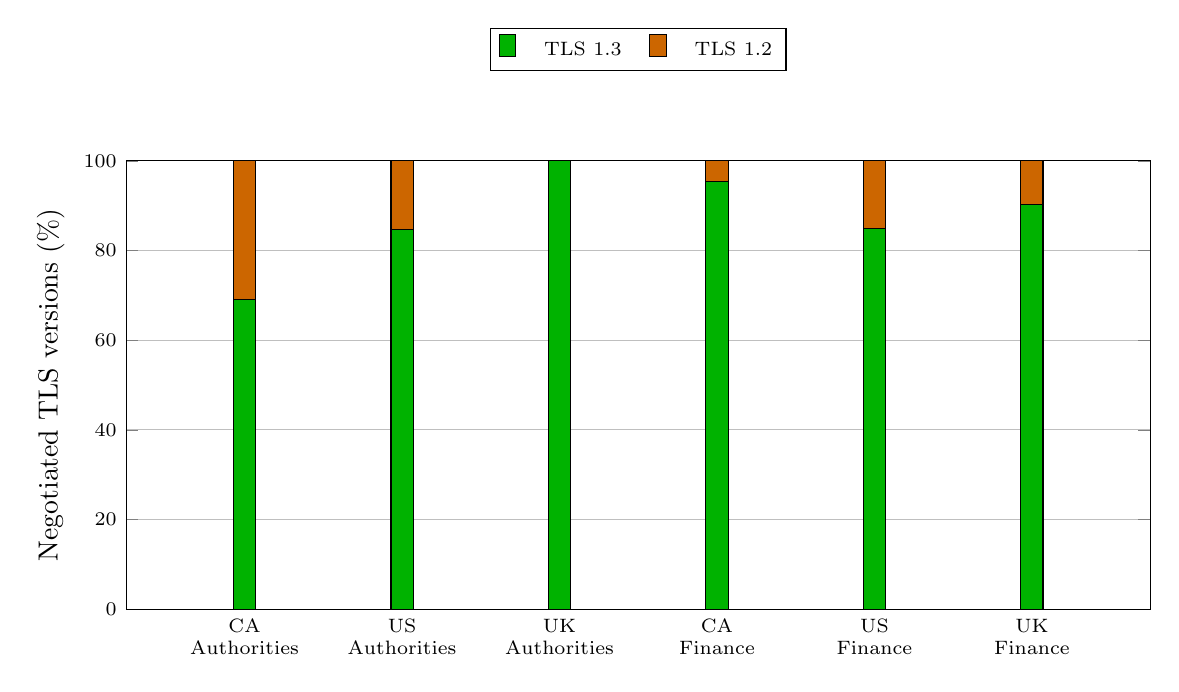
\begin{tikzpicture}
      \begin{axis}[
        ybar stacked,
        bar width=8pt,
        x=2cm,
        enlarge x limits=0.15,
        ymin=0, ymax=100,
        ylabel={Negotiated TLS versions (\%)},
        symbolic x coords={CA-Auth,US-Auth,UK-Auth,CA-Fin,US-Fin,UK-Fin},
        xtick=data,
        xticklabels={
          CA\\Authorities,
          US\\Authorities,
          UK\\Authorities,
          CA\\Finance,
          US\\Finance,
          UK\\Finance
        },
        xticklabel style={
          align=center,
          font=\scriptsize,
          text width=1.6cm
        },
        tick label style={font=\scriptsize},
        ymajorgrids=true,
        legend style={
          at={(0.5,1.20)},
          anchor=south,
          legend columns=3,
          column sep=8pt,
          font=\scriptsize,
        },
      ]

        \addplot[fill=green!70!black] coordinates {
          (CA-Auth, 69.1)
          (US-Auth, 84.6)
          (UK-Auth,100.0)
          (CA-Fin, 95.4)
          (US-Fin, 84.9)
          (UK-Fin, 90.2)
        };

        \addplot[fill=orange!80!black] coordinates {
          (CA-Auth, 30.9)
          (US-Auth, 15.4)
          (UK-Auth,  0.0)
          (CA-Fin,  4.6)
          (US-Fin, 15.1)
          (UK-Fin,  9.8)
        };

        \legend{TLS 1.3, TLS 1.2}
      \end{axis}
    \end{tikzpicture}}

    \caption{Stacked bar chart of negotiated TLS versions for authority and finance websites by country.}
    \label{fig:tls_stacked_auth_fin}
  \end{adjustbox}
\end{figure}

% ------------------------------------------------------------
% Optional (kept for reviewer requests): TLS 1.2 cipher quality
% ------------------------------------------------------------
% \paragraph{TLS 1.2 cipher suite quality (optional analysis).}
% For TLS~1.2-capable origins, cipher suite selection can provide a finer-grained view of cryptographic posture
% beyond protocol versions. If reviewers request additional detail, we can report the cipher suite negotiated
% under a forced TLS~1.2 handshake and categorize suites into guideline-derived buckets (e.g., recommended,
% sufficient, phase-out) using CCCS and allied guidance. We would then present these results as proportions
% over the subset of origins where TLS~1.2 handshakes succeed, explicitly noting that suites not covered by
% a given guideline list are ``not classified'' rather than insecure.
% 
% Where TLS~1.2 cipher suites were profiled, we classify negotiated suites into guidance-aligned categories (e.g., recommended, sufficient, phase-out) to characterize whether TLS~1.2 deployments align with modern cryptographic policy.
% This analysis is treated as complementary to protocol-version posture: protocol modernization (TLS~1.3) provides the strongest baseline, while cipher categorization helps distinguish higher- and lower-quality TLS~1.2 configurations among origins that continue to rely on TLS~1.2 negotiation.

\paragraph{HSTS deployment and policy quality}
    Finally, we evaluate whether HTTPS-capable origins deploy HSTS and whether policies meet common strength expectations. 
    Table~\ref{tab:https_hsts_quality} reports HSTS presence among HTTPS-reachable origins and summarizes configuration strength using the presence of long-lived policies (via \texttt{max-age}), subdomain coverage (\texttt{includeSubDomains}), and preload signaling. 
    A clear cross-jurisdiction gap emerges in authority datasets: Canadian authorities deploy HSTS less consistently than mandate-driven peers, and a substantial share of HTTPS-capable origins do not provide an HSTS policy at all.
    Among those that do, a subset meet strong-policy criteria (long duration with subdomain coverage), and an even smaller fraction signal preload eligibility, indicating that HTTPS is often deployed without the browser-enforced ``safety net'' that helps prevent downgrade and mixed-entry risks.

% table for hsts quality
\begin{table}[t]
  \caption{HSTS adoption and strength among HTTPS-capable origins (percent of HTTPS-ok).}
  \label{tab:https_hsts_quality}
  \centering
  \scriptsize
  \setlength{\tabcolsep}{3.5pt}
  \renewcommand{\arraystretch}{1.15}

  \begin{adjustbox}{max width=\columnwidth}
  % \resizebox{\columnwidth}{!}{%
  \csvreader[
    tabular=lrrr,
    table head=\toprule
      Dataset &
      Any HSTS (\%)&
      Strong HSTS (\%)&
      Preload (\%)\\\midrule,
    late after line=\\,
    late after last line=\\\bottomrule
  ]{./results/comparison/https_hsts/hsts_quality_summary.csv}{%
    dataset_label=\Dataset,
    pct_has_hsts_among_https_ok=\PAnyHsts,
    pct_hsts_strong_among_hsts=\PStrong,
    pct_hsts_preload_among_hsts=\PPreload
  }{%
    \Dataset &
    \PAnyHsts &
    \PStrong &
    \PPreload
  }%
  \end{adjustbox}
\end{table} 

% Discussion paragraph synthesizing transport-layer results
% Taken together, these transport-layer results show that encrypted transport is widely deployed across Canadian
% public-sector and critical-sector sites, but that Canadian authority websites exhibit weaker and less uniform
% HTTPS reachability, slower migration toward consistently negotiated TLS~1.3, and lower HSTS adoption and policy
% strength than international peers. These gaps motivate the application-layer analyses that follow, where
% defense-in-depth depends on browser-enforced policy controls and secure session handling.

\subsection{Application-Layer Hardening and Browser-Enforced Policies (Endpoint-Scoped)}
\label{sec:app_layer_hardening}
    While transport controls establish confidentiality and integrity in transit, modern web security also relies on browser-enforced policies that reduce exploitation impact and limit cross-origin abuse.
    This subsection reports adoption of browser-enforced hardening controls observable on the final, user-reached landing endpoints (i.e., after redirect resolution). 
    Because these controls are delivered as HTTP response headers and may vary across paths and applications, all results in this subsection are computed over the set of \emph{final resolved endpoints} for each dataset (Table~\ref{tab:security_headers_presence}). 

\paragraph{Security header prevalence summary}
    Table~\ref{tab:security_headers_presence} summarizes adoption of key response headers that provide defense-in-depth against common web threats and privacy leakage: \texttt{Referrer-Policy}, \texttt{X-Content-Type-Options}, \texttt{X-Frame-Options}, CSP with an explicit \texttt{frame-ancestors} directive, and \texttt{Permissions-Policy}.
    Across datasets, we observe a consistent pattern: ``low-friction'' headers that can be enabled with minimal application knowledge are deployed substantially more often than complex policy headers. 
    In particular, \texttt{X-Content-Type-Options} and \texttt{X-Frame-Options} are commonly present across sectors, whereas \texttt{Content-Security-Policy} (CSP) and \texttt{Permissions-Policy} appear far less frequently. This gap is most pronounced in the Canadian authority dataset, where the adoption of modern browser policy controls lags behind both domestic critical sectors and international peers.

% table for security headers presence
\begin{table}[t]
  \caption{Security header adoption by dataset (percent of final URIs).}
  \label{tab:security_headers_presence}
  \centering
  \scriptsize
  \setlength{\tabcolsep}{2.2pt}
  \renewcommand{\arraystretch}{1.15}

  \begin{adjustbox}{max width=\columnwidth}
  % \resizebox{\columnwidth}{!}{%
  \csvreader[
    tabular=lccccc,
    table head=\toprule
      Dataset &
      \shortstack{Referrer\\Policy} &
      \shortstack{X-Content-Type\\Options} &
      \shortstack{X-Frame\\Options} &
      \shortstack{CSP\\frame-ancestors} &
      \shortstack{Permissions\\Policy} \\\midrule,
    late after line=\\,
    late after last line=\\\bottomrule
  ]{./results/comparison/headers/security_headers_presence.csv}{%
    dataset_label=\Dataset,
    pct_referrer_policy_present=\Pref,
    pct_x_content_type_options_present=\Pxcto,
    pct_x_frame_options_present=\Pxfo,
    pct_csp_frame_ancestors_present=\Pcsp,
    pct_permissions_policy_present=\Pperm
  }{%
    \Dataset & \Pref & \Pxcto & \Pxfo & \Pcsp & \Pperm
  }%
  \end{adjustbox}
  \end{table}

\paragraph{Adoption and Configuration of Security Headers.}
    A consistent pattern emerges when contrasting ``low-friction'' headers with more ``high-complexity'' policies controls. 
    Headers such as \texttt{X-Frame-Options} and \texttt{X-Content-Type-Options} are comparatively easy to deploy and are often supported directly by common web servers, frameworks, and reverse proxies, which helps explain their broader uptake across datasets.
    However, adoption drops significantly for controls that require deliberate policy specification or iterative tuning, such as \texttt{Referrer-Policy}, \texttt{Content-Security-Policy} (CSP), and \texttt{Permissions-Policy}.
    For example, CSP often requires iterative tuning to avoid breaking legitimate resource loads, and \texttt{Permissions-Policy} requires explicit decisions about which browser capabilities should be restricted for the top-level page and embedded contexts.
    The result is a visible ``defense-in-depth gap'' in which many sites deploy baseline hardening but fail to adopt stronger policy mechanisms enforced by modern browsers.
    For example, in the Canadian authority dataset, adoption rates for \texttt{X-Frame-Options} and \texttt{X-Content-Type-Options} are in the low-to-mid 60\% range, whereas \texttt{Referrer-Policy} (17.4\%), CSP \texttt{frame-ancestors} (17.9\%), and \texttt{Permissions-Policy} (8.6\%) are observed at substantially lower rates.
    
    Because CSP policies differ widely in expressive power, rather than treating CSP as a binary indicator we specifically measure whether the policy includes \texttt{frame-ancestors}, which directly implements modern framing restrictions (clickjacking defense) at the browser level.
    Furthermore, we find that the prevalence of CSP \texttt{frame-ancestors} is significantly lower than that of the legacy \texttt{X-Frame-Options} header, indicating that many endpoints either omit CSP entirely or deploy it without the specific restrictions required for robust embedding control.
    
    \texttt{Permissions-Policy} is the least prevalent of these controls.
    This low adoption is notable because, unlike CSP, \texttt{Permissions-Policy} is a low-cost mechanism to reduce exposure to powerful browser features (e.g., camera, microphone, geolocation) and can often be deployed incrementally by disabling unused features, including for embedded third-party content.
    Single-digit adoption suggests that proactive feature restriction is not yet standard practice in public-sector and critical-sector web deployments.
    As with CSP, presence does not guarantee a restrictive configuration. However, the rarity of the header implies that most measured endpoints are not explicitly declaring feature restrictions at all.
    
    Overall, the comparative results suggest that while many services have adopted foundational hardening headers, modern browser policy mechanisms that require deliberate configuration remain under-deployed, particularly within the Canadian authority ecosystem. 
    
\subsection{Session Management and Cookie Security (Endpoint-Scoped)}\label{sec:results_cookies}

    This subsection evaluates session-management posture by analyzing cookie attributes observed on final resolved endpoints. 
    Cookies are a common mechanism for maintaining state (including authenticated sessions as well as preferences and analytics identifiers), and their security attributes are enforced by user agents rather than application logic. 
    Table~\ref{tab:cookie_security_flags} reports 
    (i) how often endpoints set cookies on their landing responses and, conditional on cookie issuance (i.e., at least one \texttt{Set-Cookie} header), 
    (ii) the prevalence of three baseline hardening attributes (\texttt{Secure}, \texttt{HttpOnly}, and \texttt{SameSite}), and 
    (iii) an aggregate ``Recommended/Sufficient'' metric capturing whether sites meet a minimal defense-in-depth cookie profile. 
    Across datasets, many landing pages do not set cookies, which is expected for informational services. Accordingly, attribute adoption is interpreted over the subset of cookie-setting endpoints. 
    Within Canadian authorities, roughly 28\% of endpoints set cookies, establishing the population for attribute-level evaluation in that sector.

    Among cookie-setting endpoints, \texttt{Secure} is typically the most common attribute, reflecting the expectation that cookies should only be transmitted over HTTPS; 
    \texttt{HttpOnly} is less consistently applied, and 
    \texttt{SameSite} is the least consistently deployed. 
    In Canadian authorities, approximately two-thirds (63.5\%) of cookie-setting sites include the \texttt{Secure} flag and about half (48.7\%) include \texttt{HttpOnly}, while only a small minority (15.7\%) set \texttt{SameSite} to at least \texttt{Lax}. 
    Critical-sector datasets (e.g., energy and finance) show different mixes of cookie issuance and attribute adoption, but none approach universal full hardening on issued cookies (e.g., the energy sector achieves only 4.9\% recommended configurations). 
    This pattern is operationally consequential because \texttt{HttpOnly} reduces exposure of session identifiers to JavaScript-accessible theft in the presence of XSS, while \texttt{SameSite} provides a browser-level mitigation against cross-site request flows that can enable CSRF-style state changes.

    To summarize whether cookie-setting endpoints achieve a minimal ``gold standard'' for baseline cookie protection, we compute the fraction of cookie-setting sites for which \emph{all observed cookies} on the landing response satisfy the triple-attribute profile: \texttt{Secure} + \texttt{HttpOnly} + \texttt{SameSite} set to at least \texttt{Lax} (reported as ``Recommended/Sufficient'' in Table~\ref{tab:cookie_security_flags}). 
    The resulting rates are extremely low: for Canadian authorities, only about 3.5\% of cookie-setting endpoints meet the recommended/sufficient profile despite much higher partial adoption of \texttt{Secure} and \texttt{HttpOnly}. 
    These attributes are foundational to session security: \texttt{HttpOnly} reduces the exposure of session identifiers to JavaScript-accessible theft (XSS), while \texttt{SameSite} provides a browser-level mitigation against cross-site request flows that can enable CSRF-style state changes.
    This gap between partial and complete hardening highlights an important operational reality: cookie security is often not governed by a uniform policy baseline, and a missing attribute can leave session identifiers exposed to common web threats even when other controls are present.

    % table for cookie security flags
\begin{table}[t]
    \caption{Cookie security flag adoption by country and sector.}
    \label{tab:cookie_security_flags}
    \centering
    \scriptsize
    \setlength{\tabcolsep}{3pt}
    \renewcommand{\arraystretch}{1.15}
    
    \begin{adjustbox}{max width=\columnwidth}
    % \resizebox{\columnwidth}{!}{%
    \csvreader[
      tabular=lllrrr,
      table head=\toprule
        Dataset &
        Sites w/ cookies (\%) &
        Secure flag (\%) &
        HttpOnly flag (\%) &
        SameSite$\ge$Lax (\%) &
        Rec./Suff. (\%) \\\midrule,
      late after line=\\,
      late after last line=\\\bottomrule
    ]{./results/comparison/headers/cookie_security_flags_summary.csv}{%
      dataset_label=\Dataset,
      pct_sites_with_cookies=\Pcookies,
      pct_secure_among_cookie_sites=\Psecure,
      pct_httponly_among_cookie_sites=\Phttp,
      pct_samesite_ge_lax_among_cookie_sites=\Psame,
      pct_rec_suff_among_cookie_sites=\Prec
    }{%
      \Dataset & \Pcookies & \Psecure & \Phttp & \Psame & \Prec
    }%
    \end{adjustbox}
  \end{table}

 \subsection{Operational Readiness and Information Governance}
 \label{sec:ops_readiness_info_gov}

    This subsection evaluates two operational dimensions that materially affect real-world risk yet are largely configuration-driven: 
    (i) whether organizations provide a standardized, machine-discoverable channel for coordinated vulnerability disclosure via \texttt{security.txt} (RFC~9116), and 
    (ii) whether publicly reachable services unintentionally expose implementation details that reduce the cost of attacker reconnaissance. 
    We operationalize the second dimension using two complementary measurements: technology-revealing HTTP response headers (e.g., \texttt{Server}, \texttt{X-Powered-By}) using OWASP-derived header lists, and disclosure in error-handling responses using our synthetic 404 probe. 
    Results are summarized in Tables~\ref{tab:securitytxt_summary}, \ref{tab:revealing_headers_summary}, and \ref{tab:error_leaks_summary}.

    Vulnerability-disclosure readiness is low across all datasets. 
    Table~\ref{tab:securitytxt_summary} shows that only a small fraction of origins publish a \texttt{security.txt} file at standard locations, indicating that standardized disclosure is not yet routine practice for public-facing services. 
    Canadian authorities are a clear outlier on the low end: only 1.1\% of Canadian authority origins (4 of 375) publish \texttt{security.txt}. 
    Among those few files, field completeness is generally good (all include \texttt{Contact} and \texttt{Expires}), but expiration hygiene is weak: only 25\% of Canadian authority files have an unexpired \texttt{Expires} value at scan time. 
    In contrast, peer authority datasets show higher adoption (e.g., U.S.\ authorities at 3.5\%) and better maintenance among the files that do exist. 
    Taken together, these results suggest that the primary limiting factor for Canadian authorities is \emph{adoption} rather than syntactic correctness once deployed.

% table for security.txt summary
\begin{table}[t]
  \caption{Security.txt adoption and field completeness by dataset.}
  \label{tab:securitytxt_summary}
  \centering
  \scriptsize
  \setlength{\tabcolsep}{2.2pt} 
  \renewcommand{\arraystretch}{1.15}

  \begin{adjustbox}{max width=\columnwidth}
  % \resizebox{\columnwidth}{!}{%
  \csvreader[
    tabular=lr rr ccc,
    table head=\toprule
      Dataset &
      $n$ orig. &
      \multicolumn{2}{c}{security.txt present} &
      Contact (\%) &
      Expires (\%) &
      Valid exp. (\%) \\
      \cmidrule(lr){3-4}
      & & Count & Share (\%) & & & \\\midrule,
    late after line=\\,
    late after last line=\\\bottomrule
  ]{./results/comparison/securitytxt/securitytxt_summary.csv}{%
    dataset_label=\Dataset,
    n_origins=\Norigins,
    n_with_securitytxt=\Nwith,
    pct_sites_with_securitytxt=\Psites,
    pct_with_contact_among_present=\Pcontact,
    pct_with_expires_among_present=\Pexpires,
    pct_valid_expires_among_expires=\Pvalid
  }{%
    \Dataset &
    \Norigins &
    \Nwith &
    \Psites &
    \Pcontact &
    \Pexpires &
    \Pvalid
  }%
  \end{adjustbox}
\end{table}

    At the same time, information exposure that facilitates reconnaissance remains widespread. 
    Table~\ref{tab:revealing_headers_summary} shows that technology-revealing headers are present on the majority of sites in most datasets, but Canadian authorities are particularly exposed: 94.4\% of Canadian authority origins emit at least one revealing header and many emit multiple such headers, indicating multi-layer stack disclosure (e.g., web server plus application framework). 
    In contrast, Canadian finance demonstrates substantially better hygiene (only 53.5\% expose any revealing header), suggesting that stronger incentives and operational practices can reduce avoidable disclosure. 
    Error-handling responses further amplify this reconnaissance surface. 
    
  % table for revealing headers summary
    \begin{table}[t]
      \caption{Distribution of technology-revealing headers by dataset.}
      \label{tab:revealing_headers_summary}
      \centering
      \scriptsize
      \setlength{\tabcolsep}{3pt}
      \renewcommand{\arraystretch}{1.15}
    
      \begin{adjustbox}{max width=\columnwidth}
      % \resizebox{\columnwidth}{!}{%
      \csvreader[
        tabular=lrrrrrc,
        table head=\toprule
          Dataset &
          $n$ sites &
          \multicolumn{4}{c}{$n$ revealing headers (\%)} &
          Any (\%) \\
          \cmidrule(lr){3-6}
          & & 0 & 1 & 2 & 3+ & \\\midrule,
        late after line=\\,
        late after last line=\\\bottomrule
      ]{./results/comparison/headers/revealing_headers_summary.csv}{%
        dataset_label=\Dataset,
        n_sites=\Nsites,
        pct_revealing_0=\Pzero,
        pct_revealing_1=\Pone,
        pct_revealing_2=\Ptwo,
        pct_revealing_3_plus=\Pthree,
        pct_with_any_revealing=\Pany
      }{%
        \Dataset &
        \Nsites &
        \Pzero &
        \Pone &
        \Ptwo &
        \Pthree &
        \Pany
      }%
      \end{adjustbox}
    \end{table}
    
    Table~\ref{tab:error_leaks_summary} shows that 47.2\% of Canadian authority origins disclose technology identifiers in error responses, and 10.7\% disclose explicit version information. 
    From an adversarial perspective, this creates a meaningful ``reconnaissance advantage'': even a single version string can significantly narrow the search space for known vulnerabilities and accelerate targeted exploitation planning. 
    Despite the prevalence of technology banners and version disclosure, we observe an important positive control across all datasets: no origins leaked raw stack traces in the error responses detected by our signatures, indicating that the most severe class of debugging output is generally suppressed in production. 
    Operationally, however, the combination of pervasive fingerprinting surface (headers and error pages) with near-absence of standardized disclosure channels (\texttt{security.txt}) is consequential: it lowers attacker effort while offering few uniform pathways for responsible reporting and coordinated remediation.

    % table for error leaks summary
    % Error Leaks Summary Table
    \begin{table}[t]
      \caption{Information leakage in HTTP error responses by dataset.}
      \label{tab:error_leaks_summary}
      \centering
      \scriptsize
      \setlength{\tabcolsep}{4pt}
      \renewcommand{\arraystretch}{1.15}
      
      \begin{adjustbox}{max width=\columnwidth}
      % \resizebox{\columnwidth}{!}{%
      \csvreader[
        tabular=lrrr,
        table head=\toprule
          Dataset &
          $n$ origins &
          Any tech leak (\%) &
          Version leak (\%) \\\midrule,
        late after line=\\,
        late after last line=\\\bottomrule
      ]{./results/comparison/error_leaks/error_leaks_summary.csv}{%
        dataset_label=\Dataset,
        n_scanned_origins=\Norigins,
        pct_any_tech_leak=\Ptech,
        pct_version_leak=\Pversion
      }{%
        \Dataset & \Norigins & \Ptech & \Pversion
      }%
      \end{adjustbox}
    \end{table}

\subsection{Cross-Sectoral and International Comparative Analysis}
\label{sec:comparative_synthesis}

    This subsection synthesizes the sectoral and cross-jurisdiction results to answer the central question of the study: whether a recommendation-driven model yields deployment outcomes comparable to mandate-driven peers, and where the largest practical gaps in defense-in-depth remain. 
    We focus on two comparisons: (i) 
    \emph{Canada public vs.\ domestic critical sectors} (authorities vs.\ finance/energy) to assess whether public-sector posture lags behind regulated or market-incentivized sectors; and 
    (ii) \emph{Canada vs.\ mandate-driven peers} (U.S.\ and U.K.) to contextualize Canadian adoption patterns against jurisdictions with enforceable HTTPS and related security requirements. 
    In the United States, HTTPS-only deployment is formalized through OMB Memorandum M-15-13 and reinforced through binding operational directives (e.g., BOD 18-01) that require concrete progress on web security controls. 
    In the United Kingdom, central government guidance similarly requires HTTPS-only service delivery and recommends HSTS configurations suitable for preloading. 
    In Canada, CCCS provides detailed technical guidance, but adoption is largely recommendation-driven rather than mandated across all public-sector web properties~\cite{omb-m-15-13,cisa_bod_18_01,cccs-itsp-40062,cccs-itsm-60005}. 

    Within Canada, the most consistent pattern across layers is that \emph{authorities underperform critical sectors} on several defense-in-depth controls. 
    Canadian finance and energy sites generally exhibit stronger transport posture (higher HTTPS reachability, greater TLS~1.3 negotiation rates, and more uniform upgrade behavior) than authority sites (Sections~\ref{sec:transport_results}--\ref{sec:reachability_resolution}). 
    More importantly, the application-layer results indicate that Canadian authorities lag in deployment of modern browser-enforced controls (notably CSP \texttt{frame-ancestors} and \texttt{Permissions-Policy}) and show extremely low ``full hardening'' cookie configurations (Sections~\ref{sec:app_layer_hardening}--\ref{sec:results_cookies}). 
    Operational readiness exhibits the sharpest disparity: Canadian authorities have near-zero adoption of \texttt{security.txt} despite pervasive information disclosure surfaces (Section~\ref{sec:ops_readiness_info_gov}). 
    Taken together, these patterns suggest that the Canadian public sector is not constrained by a lack of technical feasibility (since domestic critical sectors achieve stronger baselines), but rather by inconsistent adherence and configuration governance across authority web properties.

    Cross-jurisdiction comparisons reinforce the hypothesis that governance environments shape observable deployment. 
    Relative to U.S.\ (and U.K.\ authority datasets), Canadian authorities show lower HSTS adoption and weaker coverage of modern browser policy headers, alongside comparably low operational disclosure readiness (\texttt{security.txt}). 
    These gaps align most clearly with controls that are low-cost yet require explicit policy decisions or centralized configuration management (e.g., HSTS, disclosure channels, and policy headers). 
    This contrast is consistent with differences in enforcement regimes: U.S.\ federal policy requires secure connections for public services (OMB M-15-13) and DHS/CISA binding directives define compulsory actions and timelines for agency web security programs, while U.K.\ service guidance explicitly calls for HTTPS-only and HSTS configurations appropriate for preloading \cite{omb-m-15-13,cisa_bod_18_01}. 
    Canada’s CCCS guidance is comparable in technical substance, but without an analogous centralized mandate for uniform adoption across authority properties~\cite{cccs-itsp-40062,cccs-itsm-60005}. 
    While measurement cannot prove causality, the convergence between 
    (i) systematically higher adoption in mandate-driven peers and 
    (ii) weaker and more variable adoption in recommendation-driven environments 
    provides evidence that enforceability and accountability mechanisms are associated with more uniform deployment outcomes.

    Across multiple layers, Canadian authorities fall below most visibly on 
    (i) HSTS presence and strength, 
    (ii) modern browser policy controls (especially CSP \texttt{frame-ancestors} and \texttt{Permissions-Policy}), and 
    (iii) standardized disclosure readiness (\texttt{security.txt}). 
    In contrast, differences are smaller for foundational HTTPS availability and for negotiation of modern TLS versions among reachable origins. 
    The resulting pattern is consistent with a two-tier posture: Canada has broadly adopted baseline encryption for many services, but lags in the configuration-driven, defense-in-depth controls that transform ``HTTPS present'' into ``HTTPS enforced and hardened''. 
    This compliance gap motivates the discussion in Section~5 on how configuration standards and governance mechanisms could be translated into more uniform operational practice across Canadian public-sector web services.

\begin{table}[t]
  \caption{Statistical support for principal comparative claims.}
  \label{tab:stats_summary}
  \centering
  \scriptsize
  \setlength{\tabcolsep}{3pt}
  \renewcommand{\arraystretch}{1.15}

  \begin{adjustbox}{max width=\columnwidth}
  \csvreader[
    tabular=llccrc,
    table head=\toprule
      Theme &
      Metric &
      CA Authorities &
      Comparator &
      $\Delta$ (pp) &
      $p$-value \\\midrule,
    late after line=\\,
    late after last line=\\\bottomrule
  ]{../results/stats_analysis.csv}{%
    theme=\Theme,
    metric_label=\Metric,
    base_display=\BaseDisplay,
    comparator_dataset=\ComparatorDataset,
    comparator_display=\ComparatorDisplay,
    delta_pp_display=\DeltaPP,
    p_value_display=\PValue
  }{%
    \Theme &
    \Metric &
    \BaseDisplay &
    \shortstack{\ComparatorDataset\\\ComparatorDisplay} &
    \DeltaPP &
    \PValue
  }%
  \end{adjustbox}

  \vspace{2mm}
  \footnotesize
  \emph{Notes:} Entries report the Canadian authority estimate and comparator
  estimate as percentage with Wilson 95\% confidence interval. $\Delta$ is
  computed as Canadian authorities minus comparator (percentage points).
  Fisher's exact test was used for sparse comparisons; otherwise a chi-square
  test of independence was used. UK authority comparisons are not included in
  this summary table because their results are strongly shaped by centralized
  GOV.UK hosting rather than organization-level deployment.
\end{table}

\section{Discussion, Implications, and Limitations}~\label{sec:discussion}

    This section interprets the empirical results and distills their implications for both operators and policymakers. 
    We first summarize the study's key findings, emphasizing the main gaps that persist beyond baseline HTTPS deployment. 
    We then discuss plausible technical and organizational explanations for these patterns, including the role of governance models in shaping adoption outcomes, while avoiding causal over-claims. 
    Next, we translate the results into actionable recommendations for practitioners and public-sector stakeholderss. 
    These include recommendations we developed in collaboration with the CSA Group as part of the associated project deliverables, with the supporting report and artifacts made available in our public GitHub repository~\cite{latta_scanner_2026}. Finally, we present limitations that constrain interpretation and outline where the results should be treated as conservative lower bounds.

\subsection{Key Findings}\label{sec:key_findings}
    Our results reveal a consistent, cross-layer pattern: 
    Canadian public-sector services have largely adopted foundational transport protections, but advanced, configuration-driven defenses are uneven and often under-deployed—particularly among authority websites—relative to both domestic critical sectors and mandate-driven international peers. 
    This produces a two-tier posture in which ``HTTPS present'' is common, yet ``HTTPS enforced and hardened'' is not.

% \paragraph{Transport security is widespread, but not uniformly enforced among authorities.}
    Most datasets exhibit high levels of HTTPS reachability and frequent HTTP$\rightarrow$HTTPS upgrade behavior, indicating that encrypted transport has become a baseline expectation. 
    However, Canadian authorities show weaker and less uniform outcomes: a non-trivial share of authority origins remain unreachable over HTTPS from our vantage point, and some origins respond over HTTP without reliably supporting HTTPS, creating an enforcement asymmetry. 
    Even where HTTPS is available, browser-enforced upgrade protection remains incomplete: among HTTPS-reachable Canadian authority origins, only 59.73\% deploy HSTS, meaning that a substantial fraction do not provide the user-agent-level safety net that helps prevent downgrade and mixed-entry risks. 
    In parallel, modern TLS negotiation is common across datasets, but several populations still advertise legacy protocol support at non-zero rates, leaving unnecessary downgrade surface enabled even if modern clients negotiate TLS~1.3 or TLS~1.2 in practice.

% \paragraph{The largest posture gap occurs at the application layer (browser-enforced policies).}
    Endpoint-scoped results show that low-friction hardening headers (e.g., \texttt{X-Frame-Options} and \texttt{X-Content-Type-Options}) are adopted at moderate rates, while modern policy-driven controls drop sharply. 
    This gap is particularly visible in Canadian authorities: CSP deployment with \texttt{frame-ancestors} and \texttt{Permissions-Policy} remain rare compared to legacy headers, indicating that many services have not yet adopted the browser-enforced controls that provide stronger defense-in-depth against clickjacking and feature abuse. These findings are consistent with the operational reality that policy-heavy controls often require deliberate design decisions, staged deployment, and maintenance to avoid breaking application functionality.

% \paragraph{Cookie hardening is extremely low, even where cookies are widely used.}
    Among endpoints that set cookies, partial adoption of individual attributes (\texttt{Secure}, \texttt{HttpOnly}) is common, but complete baseline hardening remains rare. In Canadian authorities, roughly 28.2\% of endpoints set cookies, yet only 3.5\% of cookie-setting endpoints meet a minimal ``recommended/sufficient'' profile (i.e., \texttt{Secure} + \texttt{HttpOnly} + \texttt{SameSite} at least \texttt{Lax}). This gap between partial and complete hardening is operationally important: session and state cookies are only as strong as their weakest missing attribute, and inconsistent defaults leave common web threats insufficiently mitigated even when other controls are present.

% \paragraph{Operational readiness for vulnerability disclosure is near-absent where it is most needed.}
    A striking mismatch emerges between information exposure and disclosure readiness. 
    Standardized vulnerability disclosure via \texttt{security.txt} is almost absent in Canadian authorities: only 1.1\% of Canadian authority origins publish a \texttt{security.txt} file, and among those few files, expiration hygiene is often weak. 
    This matters because \texttt{security.txt} is a low-cost, configuration-only mechanism that can substantially reduce friction for responsible reporting. 
    In the absence of standardized disclosure, vulnerabilities discovered by external researchers are more likely to remain unreported or to be routed through ad hoc channels, delaying remediation.

% \paragraph{Information leakage provides a measurable reconnaissance advantage.}
    Technology-revealing response headers are pervasive across datasets and especially prevalent in Canadian authorities (94.4\% expose at least one such header). 
    Error responses further amplify disclosure: 47.2\% of Canadian authority origins leak technology identifiers in synthetic 404 responses, and 10.7\% disclose explicit version information. 
    From an adversarial perspective, these disclosures reduce reconnaissance cost and accelerate targeting. 
    At the same time, we observe one consistent positive control across datasets: raw stack traces were not exposed in the error responses detected by our signatures, indicating that the most severe class of debugging output is generally suppressed in production.

% \paragraph{Synthesis: governance and implementation incentives appear to shape uniformity.}
    Cross-sector and cross-jurisdiction comparisons converge on the same interpretation. 
    Within Canada, finance and energy often achieve stronger and more consistent posture than authorities, suggesting that regulatory pressure and operational maturity can translate guidance into practice. 
    Internationally, U.S.\ and U.K.\ authority datasets generally show more uniform adoption of several configuration-driven controls (notably HSTS and modern browser policies) than Canadian authorities. 
    While measurement alone cannot establish causality, the systematic alignment between mandate-driven environments and more uniform adoption, versus recommendation-driven environments and more variable adoption, supports the central thesis of this paper: the remaining gaps are less about technical feasibility and more about incentives, standardization, and consistent implementation.

\subsection{Explanations \& Governance Interpretation}\label{sec:explanations_governance}

    The results in Sections~\ref{sec:reachability_resolution}--\ref{sec:ops_readiness_info_gov} indicate that the largest posture gaps are concentrated in configuration-driven controls that require consistent policy decisions and ongoing maintenance (e.g., HSTS strength, modern browser policy headers, cookie hardening, and disclosure readiness), rather than in the basic availability of HTTPS. 
    Below we discuss plausible explanations for these patterns and interpret them through the lens of governance models, while emphasizing that our measurements establish associations rather than causality.

    \paragraph{Configuration complexity and deployment friction}
    A first explanation is that many of the under-deployed controls are not purely ``turnkey'' even when they are conceptually simple. 
    CSP provides a clear example: although it can materially reduce the impact of content-injection classes, practical deployment often requires iterative tuning (e.g., auditing third-party dependencies and refactoring inline scripts) to avoid breaking legitimate functionality. 
    Similarly, \texttt{Permissions-Policy} requires explicit choices about which browser capabilities should be enabled for top-level documents and embedded contexts, which may be unfamiliar to teams focused primarily on application delivery. 
    Cookie hardening also suffers from coordination challenges: \texttt{Secure} and \texttt{HttpOnly} can often be enabled centrally, but consistent \texttt{SameSite} settings can require application-level review of cross-site flows and legacy integrations.
    These frictions plausibly explain the consistent pattern observed across datasets in which low-friction headers are deployed more widely than policy-heavy controls.

    \paragraph{Decentralized ownership, vendor heterogeneity, and configuration drift}
    Public-sector web ecosystems are commonly decentralized across many departments, agencies, and contractors, and often comprise heterogeneous stacks (multiple CMSs, frameworks, CDNs, and hosting providers). 
    In such environments, security posture can degrade through configuration drift: a secure baseline may be applied to some properties but not others, or may erode over time as teams change, services are migrated, or third-party platforms are updated.
    This interpretation is consistent with two empirical observations in our data: 
    (i) the high variability of defense-in-depth controls across authority sites compared to more uniform critical-sector deployments, and 
    (ii) the strong consolidation effects observed in some datasets, where many organizations map to a small number of shared hosting origins. 
    Shared infrastructure can raise the ceiling for uniform posture when centrally configured, but it can also mask uneven adoption if some services sit outside the centralized platform or if policy baselines are not enforced consistently across all tenants.
    
    \paragraph{Measurement considerations: ``unreachable'' outcomes and defensive filtering.}
    Finally, the higher rate of scanner-observed ``unreachable'' outcomes in authority datasets is consistent with more aggressive bot mitigation, WAF/CDN filtering, or rate limiting on government domains.
    Our scanner intentionally does not attempt to bypass defenses; instead, it reports what is observable under conservative, low-interaction requests. 
    As a result, authority posture estimates may be conservative in the sense that some blocked services could implement stronger controls than we can observe.
    However, the operational implication remains relevant: aggressive filtering can also impede legitimate external monitoring and some user interactions, and it does not substitute for baseline configuration controls such as HSTS, secure cookie defaults, or disclosure readiness. 
    We therefore treat reachability and filtering behavior as part of the externally observable security posture rather than as noise to be removed.
    
\subsection{Recommendations (Operators + Policy)}\label{sec:recommendations}

The results suggest that many gaps in Canadian public-sector web posture are not driven by a lack of technical capability, but by inconsistent operationalization of well-known configuration practices. Importantly, several of the most impactful improvements can be implemented at the edge (e.g., CDN/WAF/reverse proxy) without application rewrites, while more complex policies can be deployed incrementally (e.g., introducing CSP framing restrictions first, then expanding CSP coverage). 
At a minimum, the baseline should include: HTTPS-only service delivery with strong HSTS, retirement of deprecated TLS versions and prioritization of TLS~1.3, a required set of browser-enforced hardening headers (with CSP \texttt{frame-ancestors} as the preferred framing control), default hardened cookie attributes for session/state cookies, mandatory publication of \texttt{security.txt}, and suppression of avoidable technology disclosure through response headers and error pages. Such a baseline can be implemented in stages (starting with edge-deployable controls) and integrated into routine operational monitoring to reduce configuration drift and improve uniformity across agencies and vendors. 

% \paragraph{Operator-facing recommendations (prioritized by effort and impact).}
% We recommend the following actions for operators of public-sector and critical-sector web services, prioritized by implementation effort and expected security impact:
% \begin{enumerate}
%     \item \textbf{Enforce HTTPS-only with strong HSTS.} Ensure HTTP requests are upgraded to HTTPS and deploy HSTS with a long \texttt{max-age} (at least one year) and \texttt{includeSubDomains}, pursuing preload eligibility where feasible. This provides browser-enforced downgrade resistance and reduces reliance on user behavior.

%     \item \textbf{Complete TLS modernization and retire legacy protocols.} Prefer TLS~1.3 negotiation by default and disable TLS~1.0/1.1 (and other deprecated options) to reduce downgrade surface and eliminate unnecessary attack surface. Where TLS~1.2 remains necessary, align negotiated parameters with modern policy guidance and maintain conservative cipher choices.

%     \item \textbf{Adopt modern browser policy controls incrementally.} Move beyond baseline headers by deploying (i) CSP framing restrictions via \texttt{frame-ancestors} and (ii) \texttt{Permissions-Policy} to disable unused browser features. These controls are effective defense-in-depth mechanisms and can often be introduced gradually to reduce compatibility risk. 

%     \item \textbf{Establish a uniform cookie-hardening baseline.} Ensure that cookies used for session or sensitive state are consistently set with \texttt{Secure} and \texttt{HttpOnly}, and set \texttt{SameSite} (at least \texttt{Lax}, or \texttt{Strict} where compatible). The ``full hardening'' gap observed across datasets indicates that cookie configuration is often not governed by a consistent policy and benefits from centralized enforcement (e.g., framework defaults or edge rewriting when appropriate). 

%     \item \textbf{Reduce passive fingerprinting by removing revealing headers and tightening error handling.} Remove or genericize technology-revealing headers (e.g., server and framework banners) and ensure error responses do not disclose platform identifiers or version strings. While severe debugging exposure (stack traces) is generally suppressed, the remaining disclosure signals provide an unnecessary reconnaissance advantage. 

%     \item \textbf{Publish \texttt{security.txt} and operationalize disclosure handling.} Deploy \texttt{security.txt} at standard locations with monitored contact information and an up-to-date \texttt{Expires} field. Given its low implementation cost, near-zero adoption represents a high-leverage improvement in coordinated vulnerability disclosure and time-to-remediation. 
% \end{enumerate}

% \paragraph{Policy-facing recommendations (raising baseline consistency).}
From a governance perspective, the cross-sector and cross-jurisdiction comparisons suggest that Canada's primary challenge is consistency: similar technical guidance exists, but adoption is uneven.
Accordingly, we recommend the following policy directions to raise baseline posture across public authorities: 
(i) define and enforce a minimum public-sector web baseline, 
(ii) require periodic, automated posture measurement aligned with CCCS guidance and modern web standards,
(iii) provide shared implementation support and templates, and
(iv) normalize vulnerability disclosure for public services.
% \begin{enumerate}
%     \item \textbf{Define and enforce a minimum public-sector web baseline.} Establish a small set of mandatory controls for public authority domains (e.g., HTTPS-only enforcement, strong HSTS, modern TLS configuration, baseline header posture, cookie hardening for session contexts, disclosure signaling), with clear timelines and accountability for compliance.

%     \item \textbf{Institutionalize continuous measurement and reporting.} Require periodic, automated posture measurement aligned with CCCS guidance and modern web standards. Continuous measurement reduces configuration drift and provides an objective mechanism for tracking improvement and identifying regressions.

%     \item \textbf{Provide shared implementation support and templates.} Offer centralized reference configurations (e.g., HSTS policies, CSP starter policies focusing on \texttt{frame-ancestors}, \texttt{Permissions-Policy} starter templates, cookie policy guidance) to reduce the deployment burden on smaller agencies and vendors and improve uniformity across heterogeneous stacks.

%     \item \textbf{Normalize vulnerability disclosure for public services.} Encourage or require \texttt{security.txt} adoption across government domains and ensure disclosure contacts route to teams empowered to triage and remediate issues, improving responsiveness without requiring intrusive testing.
% \end{enumerate}

As part of this project, we worked with the CSA Group to translate the empirical findings into actionable recommendations for stakeholders. 
The corresponding CSA deliverable report and supporting artifacts are available in our public repository~\cite{latta_scanner_2026}

\subsection{Limitations}\label{sec:limitations}

This study has several limitations that constrain interpretation of the results and motivate future extensions. 
First, our measurements reflect an \emph{external} vantage point and a deliberately conservative, non-invasive scanning posture. Some origins were classified as ``unreachable'' when repeated attempts failed to complete an HTTP request or TLS handshake within the ethical timeouts and stop rules. 
These outcomes may arise from genuine service unavailability or misconfiguration, but they may also reflect active WAF/CDN bot mitigation, rate limiting, geo-dependent filtering, or reputation-based blocking. 
As a result, reported adoption rates should be interpreted as a snapshot of what is observable under low-interaction requests, and in some cases may represent conservative lower bounds for controls that could be present but not externally observable due to filtering.

Second, this work measures \emph{deployment and configuration posture}, not exploitability. 
The absence of a control (e.g., HSTS, a policy header, or cookie attributes) indicates increased exposure to certain classes of web threats, but does not by itself establish the presence of a specific vulnerability or successful attack path. 
Conversely, the presence of a control does not guarantee correct implementation: for example, a site may emit a CSP header that is permissive, may apply secure cookie attributes to some cookies but not those relevant to authentication, or may deploy headers inconsistently across different application routes. 
Our results therefore represent a configuration-level benchmark rather than a penetration test or full compliance audit.

Third, endpoint-scoped measurements were performed on the \emph{final resolved landing response} only. 
Some web applications may enforce stricter controls on authenticated pages, transactional flows, or high-value endpoints (e.g., login, payments, or account portals) that are not reachable without user interaction. 
Similarly, cookie behavior can change across routes and user states, and our cookie analysis captures what is set on the landing response rather than the complete session lifecycle. 
While the landing page is a consistent and comparable surface for large-scale benchmarking, it does not exhaustively represent the security posture of all application functionality.

Fourth, our \texttt{security.txt} discovery is intentionally conservative and may undercount deployments that centralize disclosure policy on a different origin. 
We probe the standard RFC~9116 locations on each origin but do not follow cross-origin redirects for \texttt{security.txt} discovery. 
Organizations that host disclosure metadata on a shared or centralized disclosure domain may therefore be underrepresented. 
Additionally, our validity checks emphasize the presence and freshness of key fields (e.g., \texttt{Contact}, \texttt{Expires}); they do not assess whether the referenced channels are actively monitored or whether reported issues receive timely responses.

Finally, the study is cross-sectional rather than longitudinal. 
Web configurations evolve rapidly due to platform migrations, CDN policy changes, certificate renewals, and incident-driven hardening. 
Our results therefore characterize the measured window rather than long-term trends. 
Longitudinal measurement would be necessary to quantify improvement over time, identify configuration drift, and evaluate the effect of policy interventions.

% Finally, dataset construction introduces inevitable sampling and coverage constraints. 
% Although we used authoritative registries and official lists wherever possible, some sectors required sampling strategies (e.g., to manage very large populations) and some jurisdictions did not offer a single authoritative URL-complete registry for every sector (e.g., UK energy). 
% In addition, redirect-induced consolidation means that many organizational inputs may map to shared hosting platforms, which can reduce the effective diversity of measured origins in some datasets. 

\section{Conclusion and Future Work}\label{sec:conclusion_future}

This paper benchmarked the security posture of Canadian public-sector web services using a standards-aligned, non-invasive measurement methodology, with comparative baselines from the United States and the United Kingdom and additional comparison to domestic critical sectors (finance, education, and energy). By distinguishing origin-scoped transport controls from endpoint-scoped browser-enforced policies, session-cookie attributes, disclosure readiness, and information leakage surfaces, we provide a reproducible picture of what typical users and external observers encounter on the public web.

The results show that Canada has broadly adopted foundational transport protections, but that defense-in-depth remains uneven and frequently under-deployed within authority websites. 
While HTTPS is widely available and modern TLS versions are commonly negotiated by contemporary clients, enforcement and hardening controls are not consistently deployed. 
In particular, HSTS remains incomplete among Canadian authority origins that are reachable over HTTPS, standardized disclosure via \texttt{security.txt} is almost absent (1.1\% in Canadian authorities), and application-layer policy controls drop sharply relative to baseline headers. 
Cookie hardening exhibits the same pattern: although many authority endpoints set cookies, only a very small fraction meet a minimal baseline profile with \texttt{Secure}+\texttt{HttpOnly}+\texttt{SameSite} configured consistently. 
At the same time, information exposure remains pervasive: most Canadian authority origins emit technology-revealing headers and a substantial fraction disclose platform or version details in error responses, lowering the cost of attacker reconnaissance even when stack traces are correctly suppressed.

Cross-sector and cross-jurisdiction comparisons converge on a clear interpretation: the primary challenge is less about technical feasibility and more about incentives, standardization, and consistent implementation. 
Within Canada, regulated or market-incentivized critical sectors often achieve stronger or more uniform posture than authority websites, and internationally, mandate-driven environments exhibit more consistent deployment of several configuration-driven controls. 
Although measurement alone cannot establish causality, the alignment between enforceability and uniform adoption supports the central thesis of this work: closing the remaining gaps requires translating well-established guidance into consistently applied baselines, supported by accountability and continuous monitoring. 
This study provides an evidence-based baseline for that effort and a practical foundation for operators and policymakers seeking to strengthen the trust Canadians place in digital public services.

\paragraph{Future Work.}
This study motivates several extensions that would further strengthen the evidence base and increase operational utility. 
First, longitudinal measurements would quantify change over time, detect configuration drift, and enable evaluation of whether policy or operational interventions measurably improve adoption. 
Second, expanding endpoint coverage beyond landing pages (for example, authentication and other high-value workflows) would better capture how header policies and cookie attributes vary across application surfaces and user states. 
Third, multi-vantage scanning (e.g., from additional geographic regions and network environments) would help disentangle genuine unreachability from location-dependent filtering and bot-mitigation effects, improving interpretability of ``unreachable'' outcomes. 
Fourth, deeper directive-level analysis of policy headers (e.g., CSP source restrictions beyond \texttt{frame-ancestors}, and \texttt{Referrer-Policy} directive strictness) would allow posture assessment to move beyond presence/absence toward policy strength. 
Finally, integrating certificate-chain validation, certificate transparency signals, and basic DNS posture checks (e.g., CAA, DNSSEC where applicable) would provide a more holistic view of web service trust configuration beyond protocol negotiation alone.

\section*{Data \& Code Availability}
The scanner implementation, configuration templates, analysis scripts, and aggregated results used to generate the tables and figures in this paper are available in our public repository~\cite{latta_scanner_2026}. 
As part of this project, we also produced an extended technical report and recommendations deliverable in collaboration with the CSA Group, and this deliverable is included in the same repository.

\section*{Ethics Statement}
All measurements were designed to be non-invasive and configuration-focused. The scanner issued only standard HTTP(S) \texttt{GET} requests, performed protocol handshakes, and followed redirects within a bounded depth. The study evaluates externally observable configuration posture and information exposure surfaces, and it does not attempt to validate exploitability or to access non-public resources. We did not authenticate, submit forms, issue state-changing requests (e.g., \texttt{POST}), or attempt exploitation. To minimize operational impact, we enforced conservative global and per-origin concurrency limits, short client-side timeouts, and strict stop thresholds for repeated failures.


\section*{CRediT Author Statement}
Isaac Latta: Conceptualization, Methodology, Software, Data Curation, Investigation, Formal analysis, Visualization, Writing -- original draft. 
Sina Keshvadi: Conceptualization, Methodology, Supervision, Writing -- review \& editing, Project administration.

\section*{Funding}
This work was supported by the CSA Group Undergraduate Research Scholarship.

% \section*{Competing Interests}
% The authors declare that they have no known competing financial interests or personal relationships that could have appeared to influence the work reported in this paper.

\section*{Acknowledgments}
We gratefully acknowledge the support of the CSA Group Undergraduate Research Scholarship and thank CSA Group staff for their guidance during the project.

\printcredits

\bibliographystyle{cas-model2-names}
\bibliography{main}
\end{document}